%% Based on a TeXnicCenter-Template by Gyorgy SZEIDL.
%%%%%%%%%%%%%%%%%%%%%%%%%%%%%%%%%%%%%%%%%%%%%%%%%%%%%%%%%%%%%
%
%------------------------------------------------------------
%
\documentclass[a4paper,12pt,reqno]{article}
%----------------------------------------------------------
\usepackage{amsfonts}
\usepackage{graphicx}
\usepackage{geometry}
\usepackage{color}
\usepackage{amssymb,amsmath}
\usepackage{polski}
\usepackage[T1]{fontenc}
\usepackage[utf8]{inputenc}
\usepackage{caption}
\geometry{margin=1.1in}
\usepackage{wrapfig}
\usepackage{lipsum}  
\usepackage{listings}
\usepackage[toc,page]{appendix}
\usepackage{url}
\usepackage{indentfirst}
\usepackage{subcaption}
\usepackage{minted}
\usepackage{mdframed}
\usepackage{tabularx}
\usepackage{float}

\definecolor{codegreen}{rgb}{0.5, 0.09, 0.09}
\definecolor{codegray}{rgb}{0.5,0.5,0.5}
\definecolor{codepurple}{rgb}{0.58,0,0.82}
\definecolor{backcolour}{rgb}{0.94,0.94,0.94}
\definecolor{gray}{rgb}{0,0.6,0}
\definecolor{codebg}{RGB}{186, 186, 186}

% color codes
\definecolor{new}{RGB}{14, 107, 0}
\definecolor{edited}{RGB}{181, 154, 0}
\definecolor{to_change}{RGB}{255, 0, 0}
\definecolor{to_check_at_end}{RGB}{172, 0, 181}

\lstdefinestyle{mystyle}{
    backgroundcolor=\color{backcolour},  
    commentstyle=\color{codegreen},
    keywordstyle=\color{blue},
    numberstyle=\tiny\color{codegray},
    stringstyle=\color{codepurple},
	basicstyle=\footnotesize\fontfamily{cmtt}\selectfont,
    breakatwhitespace=false,         
    breaklines=true,
    captionpos=b,
	language=C++,
    keepspaces=true,                 
    numbers=left,                    
    numbersep=5pt,                  
    showspaces=false,                
    showstringspaces=false,
    showtabs=false,                  
    tabsize=2
}
 
\lstset{style=mystyle}
\lstset{literate=%
    *{0}{{{\color{gray}0}}}1
    {1}{{{\color{gray}1}}}1
    {2}{{{\color{gray}2}}}1
    {3}{{{\color{gray}3}}}1
    {4}{{{\color{gray}4}}}1
    {5}{{{\color{gray}5}}}1
    {6}{{{\color{gray}6}}}1
    {7}{{{\color{gray}7}}}1
    {8}{{{\color{gray}8}}}1
    {9}{{{\color{gray}9}}}1
}
%------------------------------------------------------------
\begin{document}

%\begin{figure}[h]
%	\centering
%		\includegraphics[width=0.40\textwidth]{logo.pdf}
%\end{figure}


\begin{center}

\thispagestyle{empty}

%UNIWERSYTET WROCŁAWSKI\\
\Large 
Uniwersytet Wrocławski\\
Wydział Fizyki i Astronomii\\
\vspace{0.8cm}
\vspace{1.8cm}

\Large Krzysztof Kukiz \\
\vspace{3.2cm}
\Large \textbf{Inteligentne powitanie na podstawie rozpoznawania twarzy} \\
\vspace{1.5cm}
Smart greeting based on face recognition
\end{center}
\vspace{3.7cm}
\begin{flushright}
\large{Praca inżynierska na kierunku \\Informatyka Stosowana i Systemy Pomiarowe \\}
\vspace{0.5cm}
\large{ Opiekun \\ dr hab. Maciej Matyka, prof. UWr}
\end{flushright}
\vspace{2.2cm}

\begin{center}
\large Wrocław, \today
\end{center}

\newpage

\tableofcontents

\newpage

%
%	Streszczenie PL
%
\begin{flushleft}
\Large \textbf{Streszczenie}
\end{flushleft}
\vspace{1cm}

Niniejsza praca przedstawia projekt systemu inteligentnego rozpoznawania osób oraz podejmowania przez system wcześniej zdefiniowanych działań, w zależności od rozpoznanej osoby. W przypadku braku rozpoznania osoby, system poda także odpowiedni komunikat głosowy oraz wizualny. 

Projekt oparty jest na Raspberry Pi 4B, na języku programowania python 3, oraz wykorzystuje elementy wydrukowane na drukarce 3D Creality Ender-3 v.2

Projekt łączy ze sobą w całość 3 warstwy niezbędne do wykonania wszystkich założonych zadań w taki sposób aby w przyszłości można było rozbudować system o kolejne funkcjonalności:

Warstwę sprzętową (Kamery, mikro-komputera, głośnika, wyświetlacza)

warstwę programistyczną odpowiedzialną za obróbkę oraz optymalizację odczytanego obrazu, interpretację pobranego obrazu oraz porównanie go z wcześniej zdefiniowaną bazą zdjęć, podjęcie decyzji o tym jakie działanie ma być podjęte oraz wygenerowanie właściwego sygnału skutkującego podjęciem określonych,

warstwę produktową w postaci dedykowanej, zaprojektowanej specjalnie dla tego projektu obudowy będącej jednocześnie opakowaniem produktu, pełniącej jego funkcje organizacyjną, ochronną, informacyjną

Głównym celem projektu było stworzenie systemu mobilnego, o jak najmniejszych wymiarach, który jest gotowy do działania natychmiast po podłączeniu zasilania.

%
%	Streszczenie EN
%
\newpage
\begin{flushleft}
\Large \textbf{Abstract}
\end{flushleft}
\vspace{1cm}

This work presents the design of a system for the intelligent recognition of persons and for the system to take predefined actions, depending on the recognised person. If the person is not recognised, the system will also give an appropriate voice and visual message.

The project is based on a Raspberry Pi 4B, the python 3 programming language, and uses components printed on a Creality Ender-3 v.2 3D printer

The project brings together the 3 layers needed to carry out all the tasks in such a way that the system can be extended in the future with further functionalities.

\begin{enumerate} % itemize
  \item A hardware layer consisting of four main components.
  \begin{itemize}
  	\item the camera, which is the signal input element and is responsible for collecting the video signal from the environment
  	\item the Rasppery Pi microcomputer, which is in charge of processing the signal from the camera, checking whether a given person's photo is in the database and issuing an appropriate message
  	\item A speaker that is an output from the system and is used to give voice announcements. The speaker plugs into a 3.5mm jack port, so any speaker can be used.
  	\item A display on which the visual part of the greeting is generated. The display is connected to the Raspberry Pi
  \end{itemize}
  \item The programming layer responsible for:
  \begin{itemize}
  	\item processing and optimisation of the read image
  	\item interpretation of the retrieved image and comparison with a predefined image database (library)
  	\item deciding on the action to be taken and generating the right signal to take the specified action
  \end{itemize}
  \item A product layer in the form of a dedicated enclosure (Etui), designed specifically for this project, performing 3 basic functions:
  \begin{itemize}
  	\item Organisational, to ensure consistent organisation of the components and their proper passive ventilation
  	\item Protective, to prevent damage to the components used in the project
  	\item Information, including basic product information
  \end{itemize}
\end{enumerate}

The aim of the project was to create a mobile system with the smallest possible dimensions, which is ready for operation as soon as the power is connected.

\newpage

%
%	Wstęp
%
\section{Wstęp} \label{section:wstep}

\subsection{Wprowadzenie}

Systemy inteligentne są stosowane obecnie na całym świecie. Znajdują coraz szersze zastosowanie w życiu codziennym każdego z nas zarówno w pracy jak i w domu. Potrafią reagować na nasze zachowania, odczytywać intencje oraz gromadzić i wykorzystywać dane, które im udostępnimy zarówno na poziomie jednostki, jak i całych grup społecznych.

W naszym codziennym życiu są elementem składowym inteligentnych budynków opartych między innymi o systemy LOXONE, KNX, AMPIO, czy też FIBARO i znacznie ułatwiają codzienne czynności poprzez sterowanie klimatem, ogrzewaniem, rekuperacją, czy też podlewaniem ogrodów, sprzątaniem, a nawet optymalnym wykorzystaniem energii elektrycznej.

Systemy inteligentne pomimo swoich kosztów zdobywają coraz większą popularność nie tylko w zastosowaniach profesjonalnych, ale także w zastosowaniach prywatnych i mogą być oparte zarówno o infrastrukturę przewodową (patrz rys. \ref{kable}), jak i mogą być oparte na rozwiązaniach bezprzewodowych.

\begin{figure}[H]%
\centering
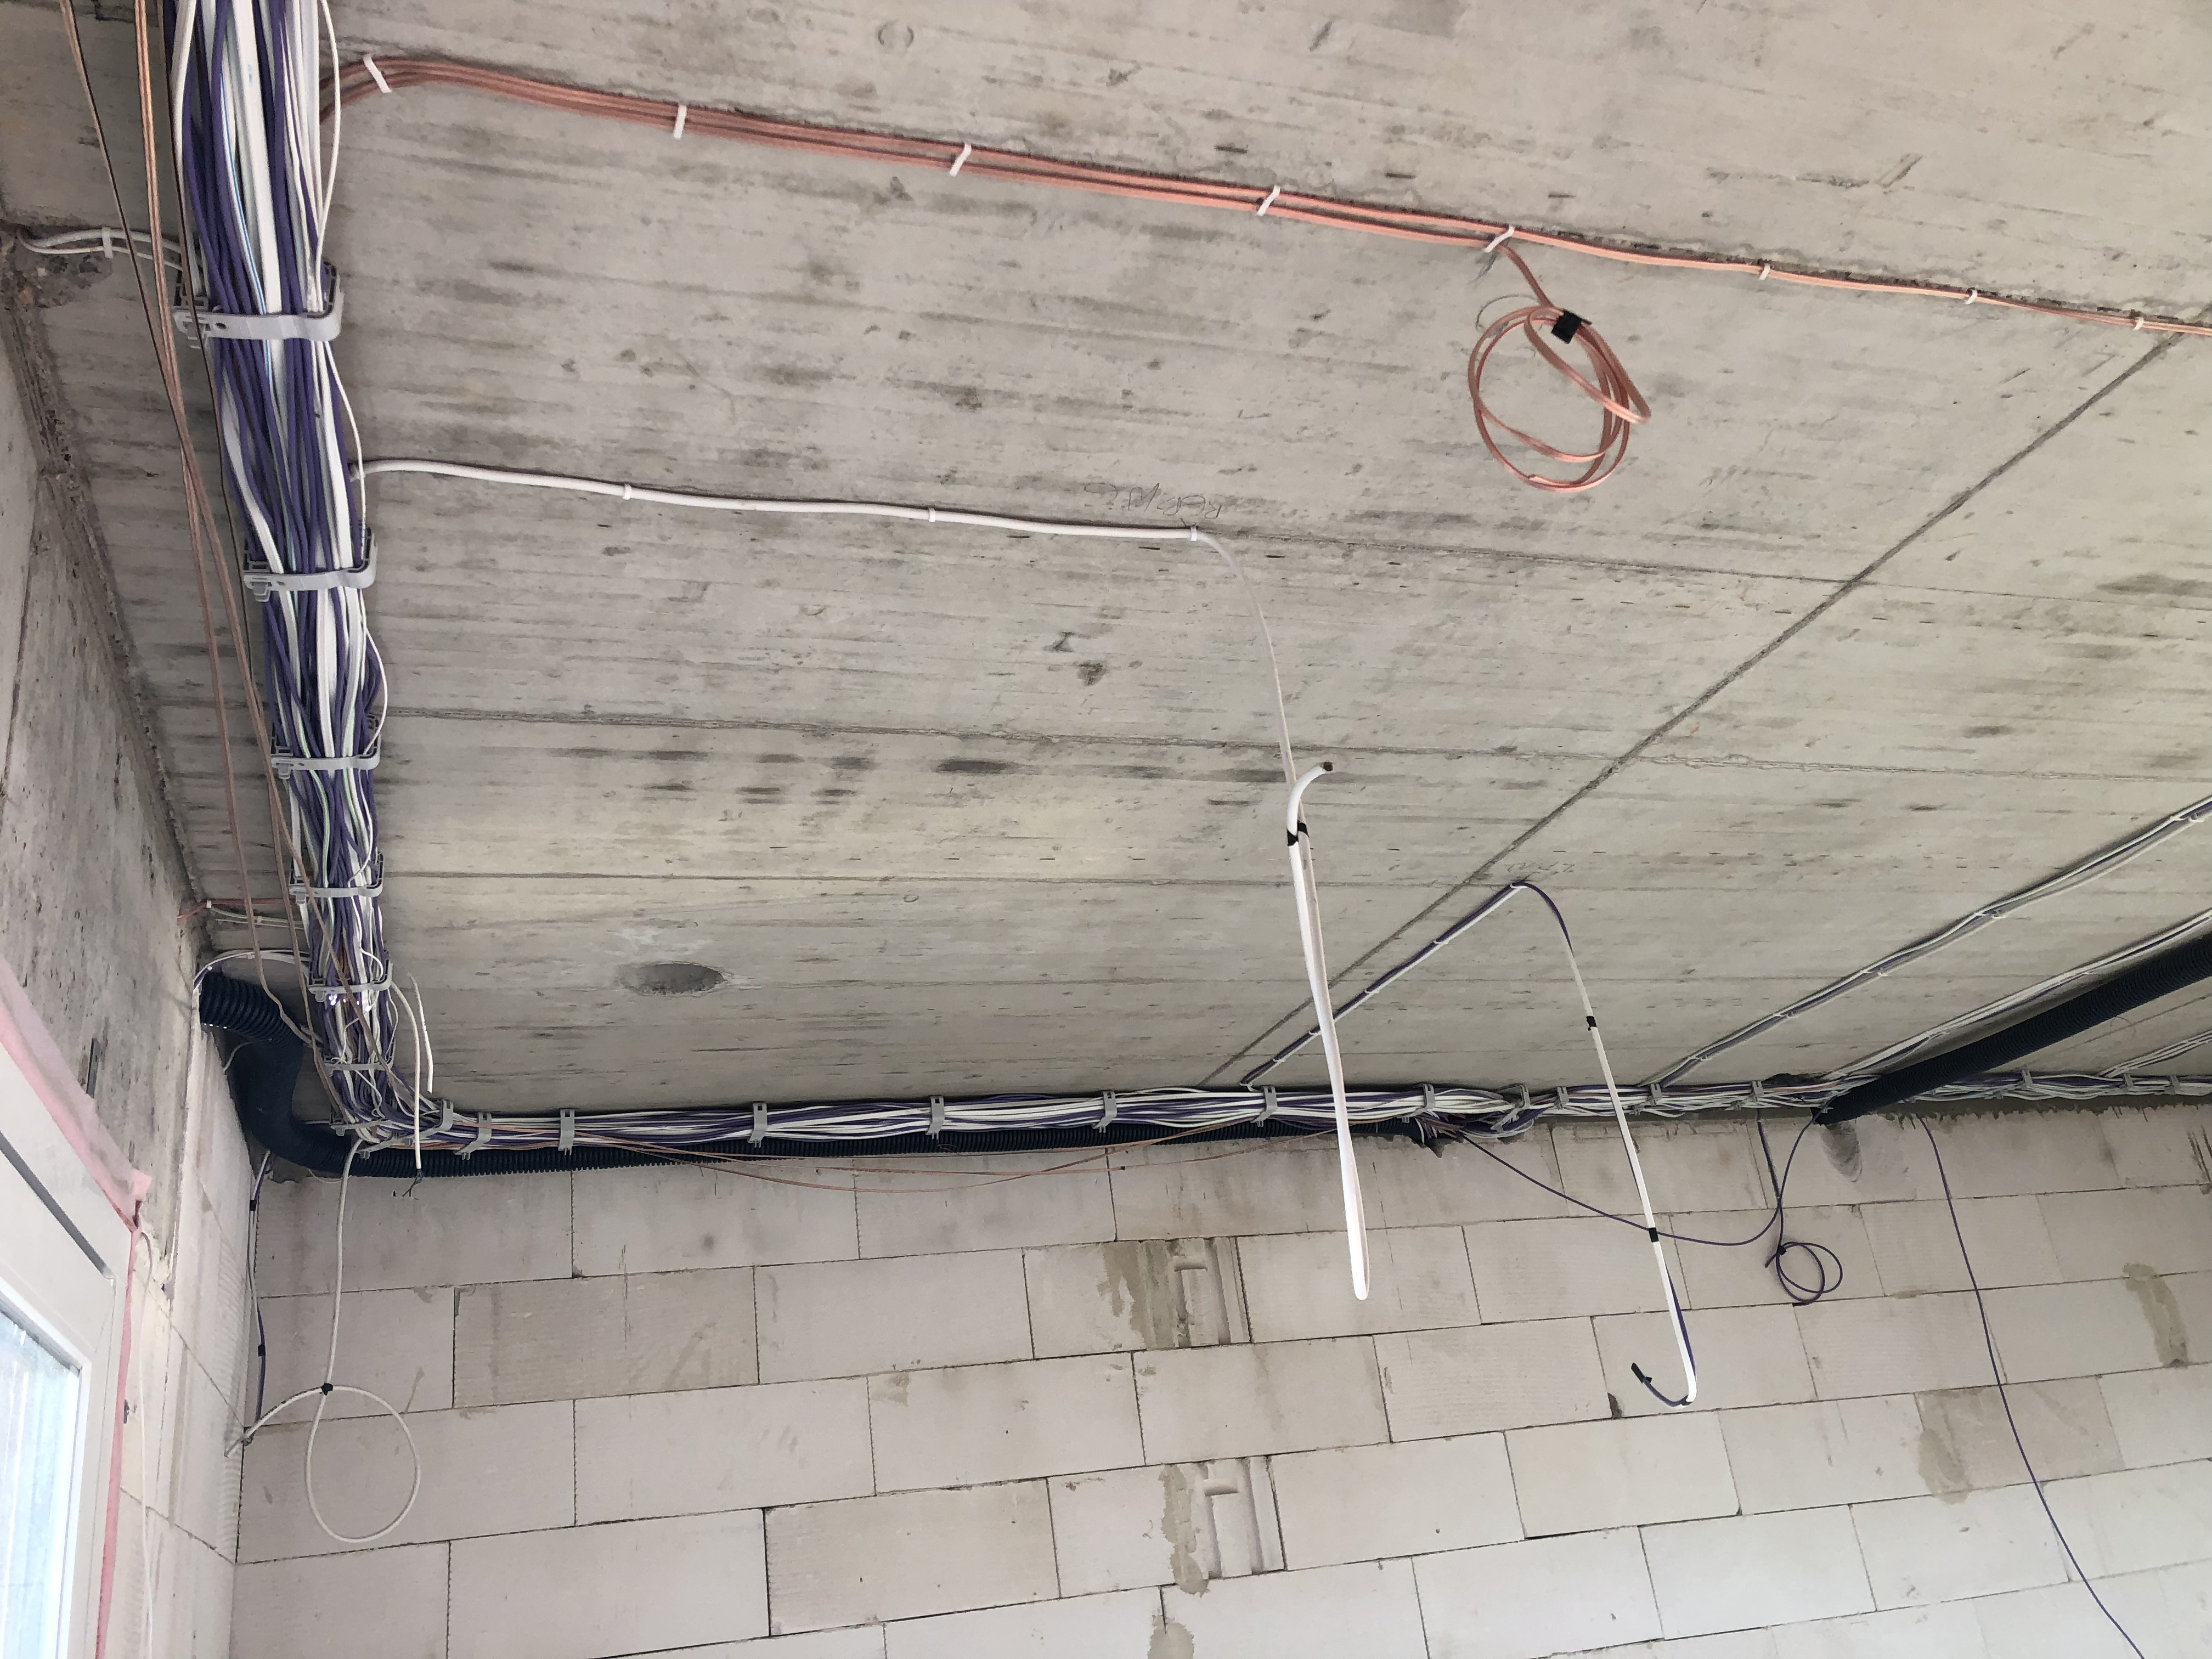
\includegraphics[width=0.8\columnwidth]{imgs/domkable.jpg}
\caption{Przykład okablowaniem domu inteligentnego. \label{kable}}
\quad
\end{figure}

Żaden system nie posiada jednak wszystkich funkcjonalności, które są niezbędne danemu użytkownikowi. W większości z nich brakuje mobilnego systemu pozwalającego na rozpoznanie osób oraz podjęcia konkretnych działań w zależności od osoby, która została zidentyfikowana.

System inteligentnego rozpoznawania osób, który jest tematem niniejszego projektu, pozwala właśnie na identyfikację osób wchodzących do pomieszczenia na podstawie zapisanej wcześniej bazy zdjęć oraz powitanie ich indywidualnym komunikatem zarówno głosowym, jak i wizualnym.

Do realizacji projektu wykorzystałem micro-komputer Raspperry Pi 4B oraz język programowania Python 3. Jako elementu wejściowego sygnału użyłem kamery Raspberry Pi Camera HD v2 8MPx zgodnej z Raspperry Pi 4B, oraz najzwyklejszego głośnika pod wejscie jack 3,5mm

\subsection{Cel i zakres pracy}

Celem głównym projektu jest stworzenie prototypu inteligentnego, mobilnego systemu rozpoznawania osób, na podstawie wcześniej zgromadzonej bazy zdjęciowej, a także wygenerowanie unikatowego powitania głosowego oraz wizualnego w zależności od rozpoznanej osoby.

Celami szczegółowymi projektu są wybór technologii sprzętowej, wybór technologii programistycznej oraz zaprojektowanie i wykonanie obudowy prototypu, mieszczącej wszystkie elementy projektu

Praca swoim zakresem obejmuje zarówno tematykę z dziedziny elektroniki, informatyki projektowania oraz prototypowania 3D.

W zakresie elektroniki wykorzystane zostały układy i sensory zgodne z płytką Rasppery 4B, w zakresie informatyki napisany został program w języku Python 3 i wykorzystujący do realizacji zadań dostępne biblioteki, natomiast w zakresie prototypowania z wykorzystaniem druku 3D, użyta została drukarka 3D Creality Ender v2 oraz materiał EASY PET-G. Do celów zaprojektowania obudowy wykorzystano program SOLIDWORKS.

Projekt z jednej strony pokazuje, że połączenie wiedzy z zakresu elektroniki, informatyki oraz projektowania dostarcza każdemu studentowi odpowiednią wiedzę oraz umiejętności, do wykonania prototypu od fazy projektowej do fazy praktycznego zastosowania,  z drugiej udowadnia, że wiedza ta pozwala na wykonania projektu z wykorzystaniem elementów ogólnodostępnych na rynku.

\subsection{Struktura pracy} % tutorial jak prrace czytać

Rozdział pierwszy zawiera wstęp, wprowadzenie, opis celu oraz zakresu pracy, a także strukturę pracy. Znajdują się w nim podstawowe informacje opisujące główne elementy składowe projektu, oraz umożliwia szybkie zapoznania się z projektem na poziomie ogólnym

Rozdział drugi zawiera założenia odnośnie szczegółowych wymagań stawianych projektowi i umożliwia zrozumienie koncepcji projektu zarówno na poziomie ogólnym i bardziej szczegółowym.

Rozdział trzeci zawiera zestawienie założone funkcjonalności projektu, które będą zaimplementowane w projektowanym systemie oraz sposób korzystania z tych funkcjonalności.

Rozdział czwarty zawiera szczegółowy opis warstwy sprzętowej z wyszczególnieniem użytych w projekcie podzespołów oraz ich parametrów. Znajdują się w nim szczegółowe opisy użytej do projektu kamery, mikrokomputera Raspberry Pi, głośnika oraz ekranu służącego do komunikacji z użytkownikiem.

W rozdziale piątym znajduje się opis warstwy programistycznej projektu z uzasadnieniem wyboru języka Python jako języka programowania użytego w projekcie, opis zastosowanych bibliotek, algorytm oraz główne elementy kodu odpowiedzialne za działanie całego projektu.

W rozdziale szóstym znajduje się opis warstwy produktowej projektu z opisem użytej technologii druku 3D, kroków projektowania obudowy, procesu wykonania obudowy oraz szczegółów samej obudowy.

W rozdziale siódmym opisane zostały kwestie związane z samą realizacją projektu, napotkane problemy oraz sposoby jakimi problemy zostały rozwiązane. Omówiono także potencjalne możliwości rozbudowy projektu o kolejne funkcjonalności i zastosowania.

W rozdziale ósmym zawarto wnioski oraz „Lessons learned” z wykonanego projektu. Stanowią one podstawę do dalszego doskonalenia podejścia przy kolejnych projektach.

\newpage
\section{Wymagania stawiane projektowi} \label{section:wymagania}

W celu realizacji pracy w pierwszej kolejności zostały określone wymagania, które stanowiły punkt docelowy projektu, jaki należało osiągnąć w ramach prac projektowych, a następnie pozwoliły na zaplanowanie drogi dojścia do założonego celu.

Na podstawie założonego celu zostały określone kroki milowe, które należało osiągnąć. Kroki te dzieliły cały projekt na mniejsze etapy, z jednej strony pozwalające na lepszy nadzór nad postępami pracy, oraz natychmiastowe określenie punktów stanowiących problem i wstrzymujących postępy, a z drugiej strony pozwalały na elastyczne reagowanie i zmiany projektowe bez konieczności zmian poprzednich etapów.

Takie podejście miało zapewnić iż ewentualny błąd popełniony na dalszych etapach nie będzie miał wpływu na etapy poprzednie projektu.

\begin{figure}[H]%
\centering
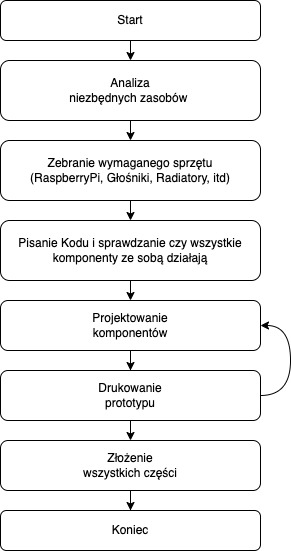
\includegraphics[width=0.5\columnwidth]{imgs/etapy.drawio.jpg}
\caption{Etapy prac projektowych. \label{etapypracy}}
\quad
\end{figure}

\subsection{Wymagania dla prototypu}

W ramach realizacji projektu zostały określone następujące wymagania dla prototypu.

\begin{itemize}
	\item \textbf{Mobilność.} Głównym założeniem projektu jest mobilność prototypu. Oznacza to, iż będzie posiadał wymiary oraz wagę umożliwiającą łatwe przenoszenie w dowolne miejsce.
	\item \textbf{Łatwość zasilania.} Prototyp powinien mieć możliwość zasilania z ogólnodostępnej sieci 230V, tak aby istniała możliwość stałego podłączenia do gniazda elektrycznego. Opcjonalnie założono, że prototyp będzie posiadał możliwość podłączenia do zasilania z powerbanku, tak aby mógł znaleźć zastosowanie w miejscach, w których dostęp do sieci elektrycznej jest utrudniony.
	\item \textbf{Dostępność.} Prototyp zostanie wykonany ze standardowych elementów dostępnych na rynku polskim.
	\item \textbf{Relatywnie niski koszt.} Wykonanie prototypu powinno mieścić się w kwocie nie większej niż 1000 zł
	\item \textbf{Łatwość obsługi.} Prototyp będzie umożliwiał obsługę bez konieczności znajomości zagadnień technicznych. Zadaniem użytkownika będzie jedynie wprowadzenie bazy zdjęć do określonego folderu, oraz uruchomienie dwóch programów:
		\begin{itemize}
			\item program "zapisujący" zdjęcia twarzy do zakodowanego pliku,
			\item główny program rozpoznający osoby przechodzące przed kamerą
		\end{itemize}
	i odpowiednie nakierowanie kamery prototypu.
	\item \textbf{Łatwość rozbudowy.} Platforma na jakiej zostanie zbudowany prototyp będzie pozwalała na jego łatwą rozbudowę.
	\item \textbf{Łatwość programowania.} System będzie oparty o jeden z popularnych języków programowania, w którym dostępne są biblioteki niezbędne do realizacji wszystkich zadań, tak aby użytkownik mógł skorzystać z dostępnych standardowych rozwiązań programistycznych, bez ponoszenia dodatkowych kosztów.
\end{itemize}

\subsection{Wymagania dla procesu projektowego}

W celu wykonania prototypu zostały określone następujące wymagania dla procesu projektowego.

\begin{itemize}
	\item \textbf{Elastyczność.} Projekt zostanie podzielony na mniejsze etapy, tak aby w każdej chwili istniała możliwość modyfikacji założeń lub działań przy jednoczesnym zapewnieniu realizacji założonych celów.
	\item \textbf{Dostępność narzędzi.} Dla każdego etapu projektu zostaną użyte narzędzia dostępne na rynku, tak aby uniknąć konieczności projektowania samych narzędzi.
	\item \textbf{Przejrzystość.} Na każdym etapie status prac będzie łatwo weryfikowalny aby zidentyfikować potencjalne przeszkody mogące powodować opóźnienie realizacji projektu.
	\item \textbf{Backup.} W celu uniknięcia utraty danych lub kodu źródłowego zostanie wykorzystane repozytorium Git. Wersja dostępna online znajduje się na Githubie \cite{moj_github}
\end{itemize}

\newpage
\section{Oczekiwane funkcjonalności projektu} \label{section:oczekiwania}

W ramach realizacji projektu zostały zaimplementowane następujące funkcjonalności.

\begin{itemize}
	\item \textbf{Zapis zdjęć twarzy} do postaci numerycznej. Użytkownik do imiennych folderów wprowadza zdjęcia twarzy osoby (np. zdjęcia Jana wrzucam do folderu "Jan Nowak") i uruchamia program encodujący zamieniając zdjęcie twarzy na wartości liczbowe.
	\item \textbf{Użycie syntezatora mowy.} System korzysta z syntezatora mowy w celu dodania deflautowego powitania do pliku .mp3.
	\item \textbf{Wykrycie osoby.} System skanuje wybrany obszar przestrzeni i wykrywa czy w nadzorowanym obszarze znajduje się osoba. W przypadku wykrycia aktywowane są kolejne kroki programu. System pomija zwierzęta oraz przedmioty.
	\item \textbf{Skanowanie  twarzy.} Po wykryciu obiektu kamera koncentruje się na twarzy wykrytej osoby i encoduje twarz w celu porównania z lokalną bazą.
	\item \textbf{Porównanie (Identyfikacja) twarzy.} System porównuje zencodowane zdjęcia z wcześniej zencodowanymi zdjęciami znajdującymi się wbazie danych. System przekształca dane wejściowe do macierzy liczb. Funkcja z biblioteki porównuje wszystkie macierze i patrzy czy dana osoba istnieje.
	\item \textbf{Komunikat głosowy.} Z puli powitań plików .mp3 (domyślnie jeden, można wrzucić własne dzwięki), program losuje jeden i go odpala (W przypadku gdy jest tylko jeden plik, losowanie się nie odbywa).
	\item \textbf{Komunikat wizualny.} Na ekranie dodatkowo pojawia się komunikat graficzny z imieniem i nazwiskiem (Patrz rys. \ref{komunikatgraficzny:komunikatgraficzny}\subref{komunikatgraficzny:rozpoznana}). W przypadku wykrycia osoby nieznanej pojawia się stosowny komunikat (Patrz rys. \ref{komunikatgraficzny:komunikatgraficzny}\subref{komunikatgraficzny:NIErozpoznana})
\end{itemize}
\begin{figure}[H]%
	\centering
	\begin{subfigure}{.5\textwidth}
		\centering
		
\includegraphics[width=0.8\linewidth]{imgs/testy_rozpoznana.jpg}
		\caption{Rozpoznanej osoby.}	
		\label{komunikatgraficzny:rozpoznana}
	\end{subfigure}%
	\begin{subfigure}{.5\textwidth}
		\centering
		
\includegraphics[width=0.8\linewidth]{imgs/testy_NIErozpoznana.jpg}
		\caption{NIE rozpoznanej osoby}
		\label{komunikatgraficzny:NIErozpoznana}
	\end{subfigure}%
\caption{Komunikaty graficzne}
\label{komunikatgraficzny:komunikatgraficzny}
\end{figure}

Powyższe funkcjonalności pozwalają na realizację funkcji

\begin{itemize}
	\item powitania
	\item nadzór obszaru
\end{itemize}

Przykłady realizacji funkcji powitania:
\begin{itemize}
	\item "Urządzenie rozpoznała Jana, który ma 3 wersje powitania. Program wylosuje i powie jedno z:"
	\begin{itemize}
		\item "Cześć Jan, miło Cię widzieć"
		\item "Witaj w domu Janek"
		\item "Panie Janie, Panie Janie ..." % ♫ ... ♫
	\end{itemize}
	\item "Urządzenie rozpoznała Adama Nowaka, który ma tylko podstawowe pytanie. Program bez losowania odrazu je wybierze i powie:"
	\begin{itemize}
		\item "Witaj Adam Nowak"
	\end{itemize}
	\item Dla nierozpoznanej osoby możemy mieć tylko domyślne przywitanie, ale możemy dać ich więcej. Program zachowa się analogicznie do wcześniej wymienionych przypadków:
	\begin{itemize}
		\item "Witaj nieznajomy"
		\item "Witamy w domostwie Nowaków"
	\end{itemize}
\end{itemize}

\newpage
\section{Warstwa sprzętowa} \label{section:warstwa_sprzetowa}

W ramach warstwy sprzętowej projekt składa się z 4 elementów. Kamery, mirko-komputera Raspberry Pi, głośnika oraz ekranu.

Podstawą systemu jest Raspberry Pi, do którego podłączone są wszystkie elementy wejściowe oraz wyjściowe prototypu, tak aby stanowiły spójną całość. W ten sposób przygotowana warstwa sprzętowa będzie następnie oprogramowana (patrz rozdział ~\ref{section:warstwa_programistyczna}) oraz zabezpieczona obudową pełniącą jednocześnie funkcje opakowania (patrz rozdział ~\ref{section:warstwa_produkcyjna})

\subsection{Kamera jako element wejściowy}

Spośród dostępnych kamer w projekcie zastosowano kamerę  HD v2 8MPx dedykowaną do mikrokomputera Raspberry Pi. Urządzenie posiada matrycę o rozdzielczości 8 Mpx, wspiera tryb HD 1080p, 720p oraz 640 x 480p oraz jest w stanie wykonywać zdjęcia w wyższej rozdzielczości 3280 x 2464 px.

Aby uniknąć potencjalnych problemów w przesyle sygnału zastosowano oficjalny moduł Raspberry Pi Camera HD v2, który jest całkowicie zgodny ze sterownikami, dostarczanymi wraz z systemem Raspberry Pi OS.

Dzięki takiemu rozwiązaniu możliwe jest jednocześnie szerokie wsparcie w zakresie dokumentacji, tutoriali oraz bibliotek programistycznych.

\begin{figure}[H]%
\centering
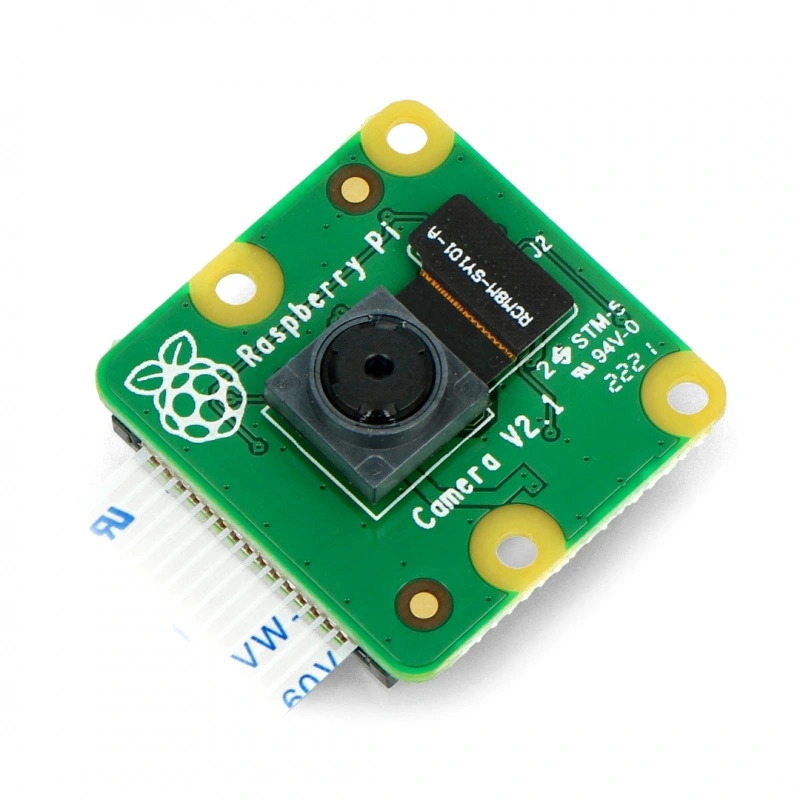
\includegraphics[width=0.8\columnwidth]{imgs/camera.jpg}
\caption{Kamera HD \cite{img_cam} \label{kamera}}
\quad
\end{figure}

Parametry kamery

\begin{itemize}
	\item HD 1080p / 30 fps,
	\item 720p / 60 fps,
	\item 640 x 480p / 90 fps.
\end{itemize}

\subsection{Płyta Raspberry Pi}

Spośród dostępnych modeli Raspberry Pi do projektu wykorzystano model w wersji 4B, który charakteryzuje się zwiększoną pojemnością pamięci RAP (4GB) oraz wydajniejszym procesorem (Broadcom BCM2711) quad-core 64-bitowy ARM-8.

Posiada on dwa złącza microHDMI, dwa złączami USB 3.0 i 2 złącza USB 2.0. Zasilanie realizowane jest przez złącze USB C.

Mikrokomputer wyposażony jest także w dwuzakresowe WiFi 2,4 GHz i 5 GHz, Bluetooth w standardzie 5, oraz port Ethernet o prędkości do 1000 Mb/s.

\begin{figure}[H]%
\centering
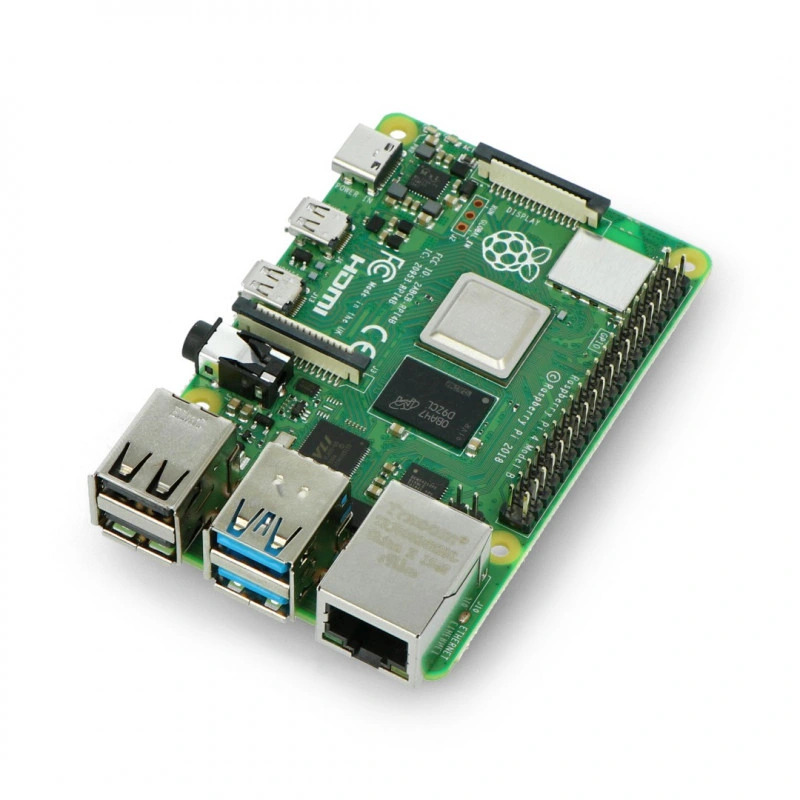
\includegraphics[width=0.8\columnwidth]{imgs/raspberrypi4.jpg}
\caption{Raspberry Pi 4B \cite{img_rp4b} \label{rp4b}}
\quad
\end{figure}

Specyfikacja techniczna

\begin{itemize}
	\item Pamięć RAM - 1GB, 2GB lub 4GB LPDDR4
	\item Procesor - Broadcom BCM2711, quad-core Cortex-A72 (ARM v8) 64-bit SoC @ 1.5GHz
	\item GPIO - 2 x 20 pin, raster 2,54 mm (wstecznie kompatybilne)
	\item Przesył danych
		\begin{itemize}
			\item 2.4 GHz oraz 5.0 GHz IEEE 802.11b/g/n/ac
			\item LAN Gigabit Ethernet
			\item Bluetooth 5.0
			\item BLE
			\item 2 × USB 3.0
			\item 2 × USB 2.0
			\item mini jack 3.5mm
		\end{itemize}
	\item Obraz i dźwięk - 2 × microHDMI (wsparcie 4k)
	\item Złącza
		\begin{itemize}
			\item DSI dla wyświetlaczy
			\item CSI dla kamer
			\item Komunikacja - UART, SPI, I2C, GPIO
		\end{itemize}
	\item Multimedia
		\begin{itemize}
			\item H.265 (4Kp60 decode)
			\item H.264 (1080p60 decode, 1080p30 encode)
			\item OpenGL ES, 3.0 graphics
		\end{itemize}
	\item Karta pamięci - microSD
	\item Systemy operacyjne - Linux Raspbian, Windows 10 loT i wiele innych
	\item Temperatura pracy - 0–50°C
	\item Zasilanie - złącze USB C minimum 5V/3A, złącza GPIO minimum 5V/3A
PoE przy zastosowaniu dedykowanej nakładki
	\item Wymiary - 85 x 56 x 17 mm
\end{itemize}

\subsection{Głośnik, jako element wyjściowy}

W zakresie komunikatów głosowych w projekcie został zastosowany głośnik LOGIC CONCEPT LS-09.

Logic Concept LS-09, to zestaw dwóch głośników, które można podłączyć zarówno do komputerów stacjonarnych, laptopów, jak i różnego rodzaju urządzeń multimedialnych. Głośniki charakteryzują się niewielkimi rozmiarami, co było jednym z warunków niezbędnych do realizacji projektu.

Każdy głośnik o mocy 3W. Dzięki niewielkim rozmiarom oraz lekkiej konstrukcji w łatwy i wygodny sposób można je przetransportować.

Zasilane realizowane jest poprzez kabel USB podłączany do Raspberry pi.

\begin{figure}[H]%
\centering
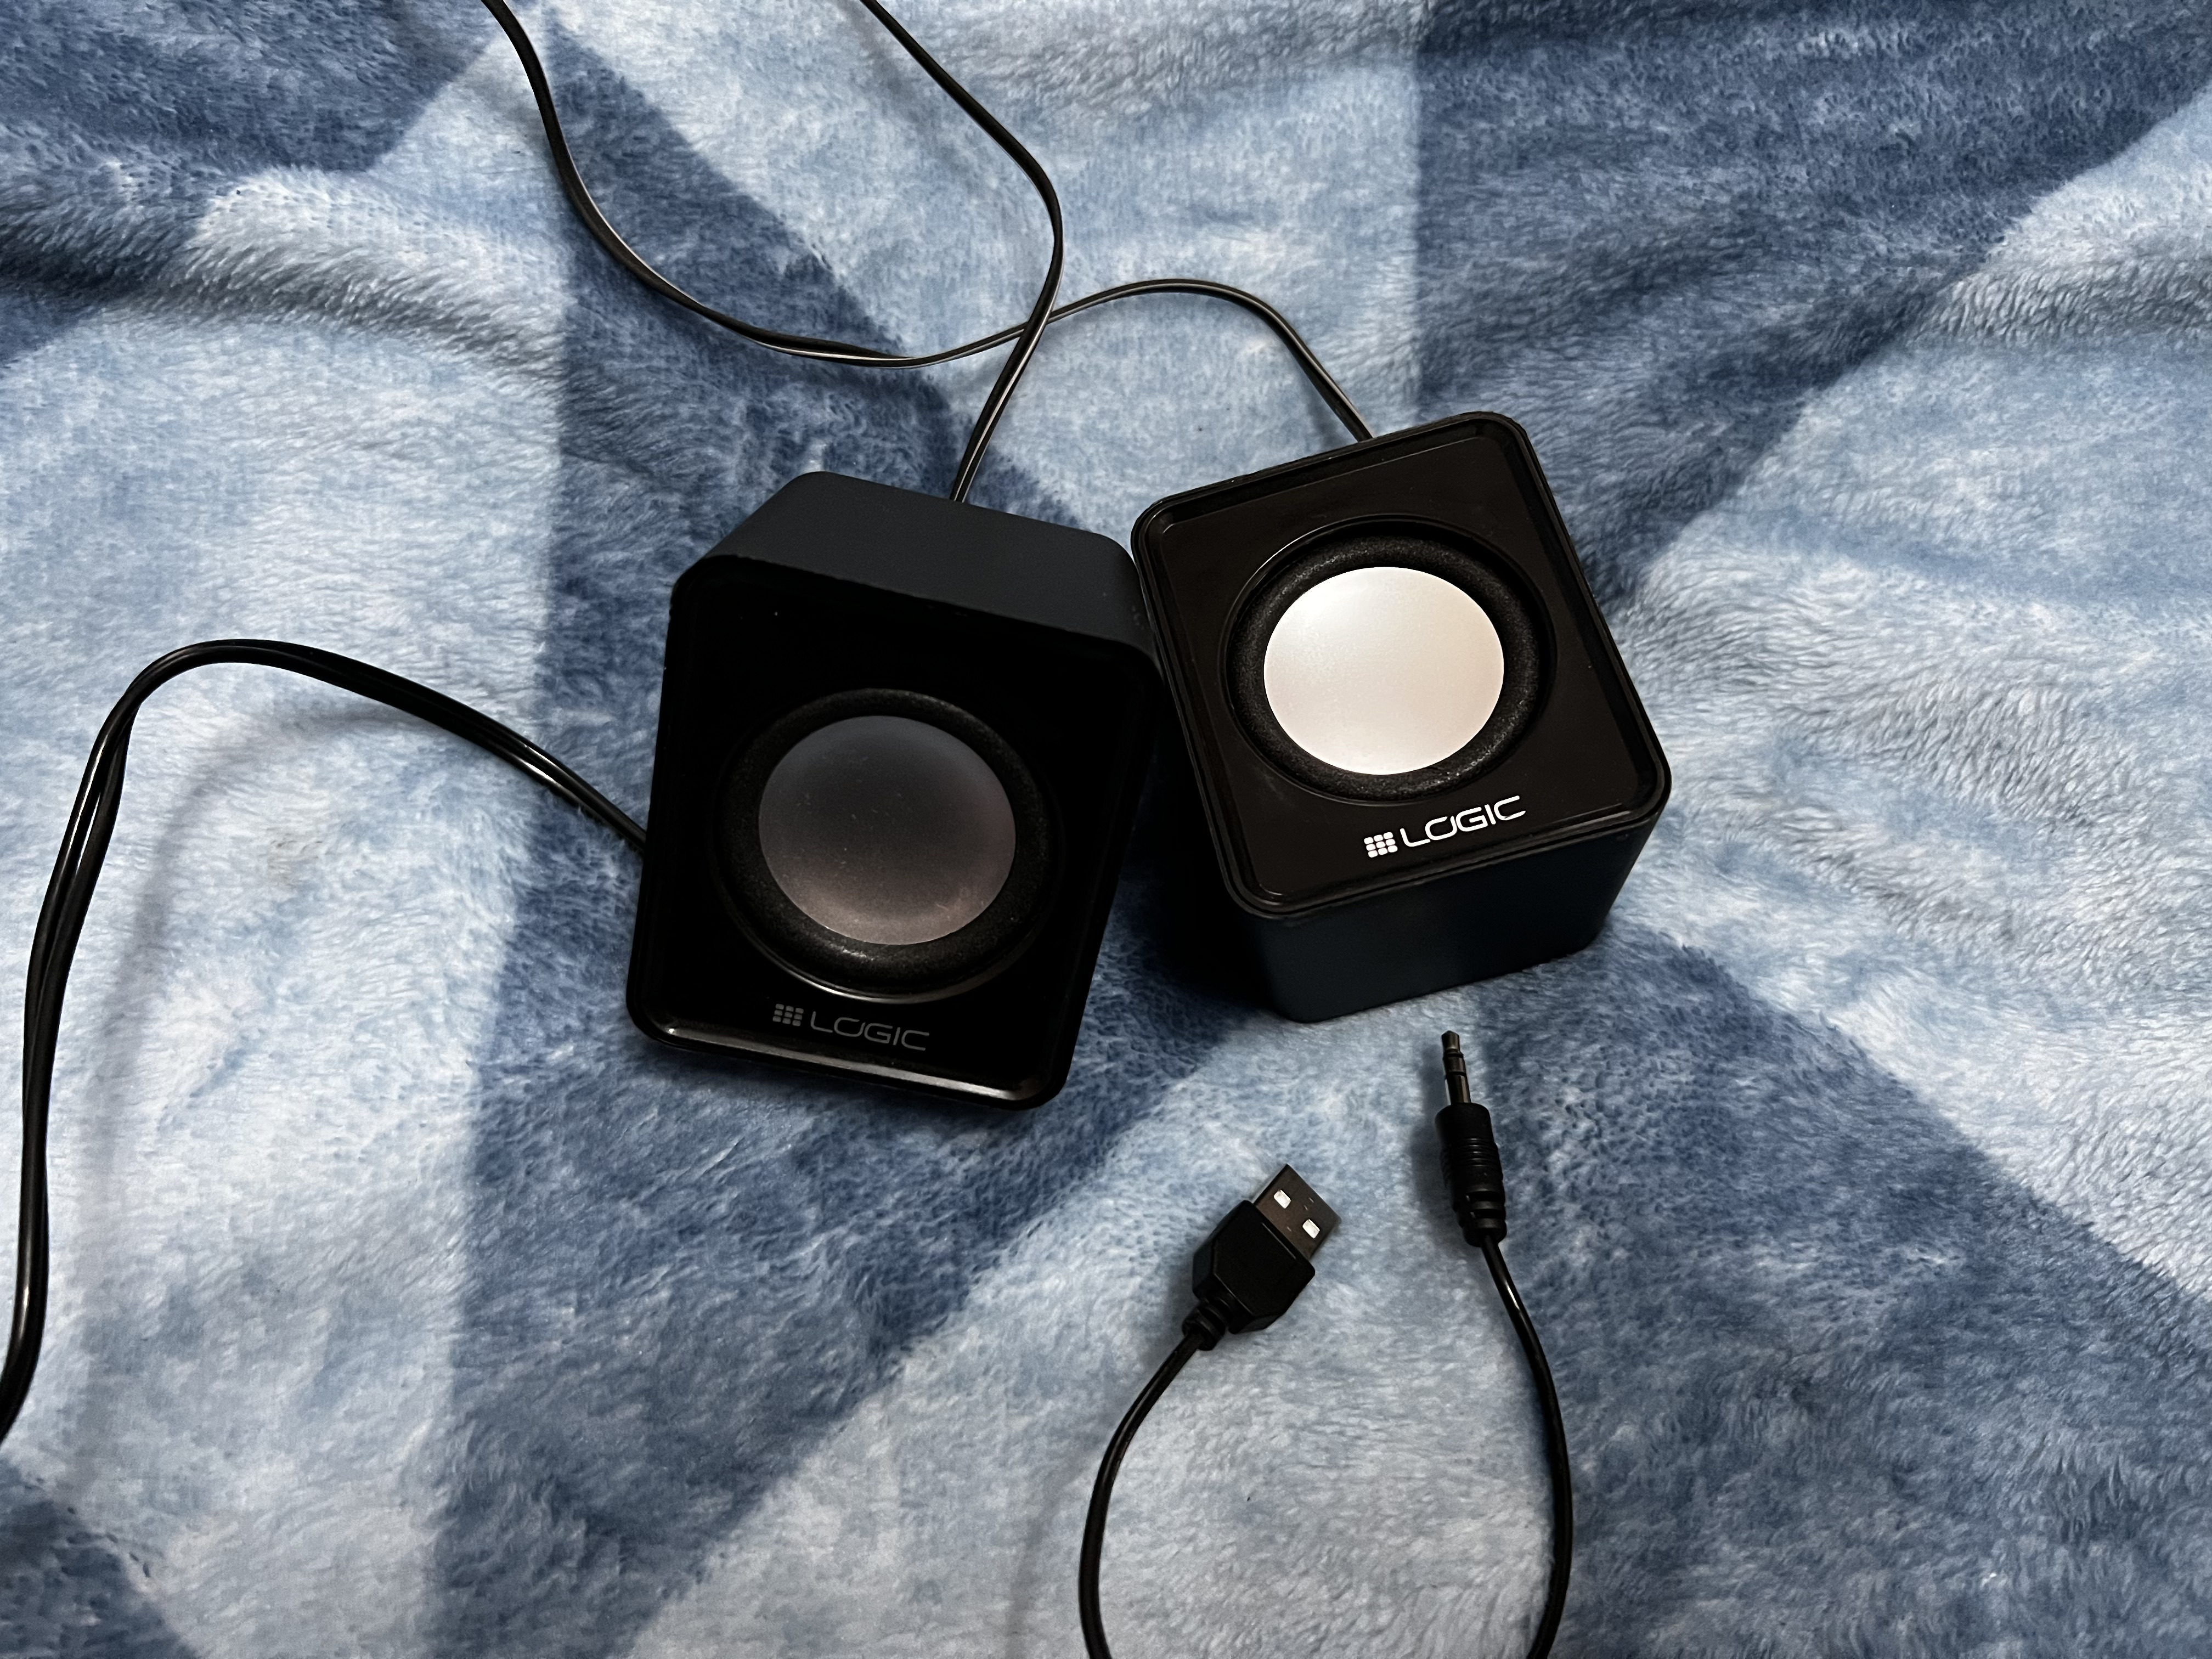
\includegraphics[width=0.8\columnwidth]{imgs/glosnik.jpg}
\caption{Głośniki LOGIC CONCEPT LS-09  \label{glosnik}}
\quad
\end{figure}

\subsection{Ekran, jako element wyjściowy}

W projekcie został zastosowany ekran Ekran dotykowy Waveshare 9904. Jest to ekran rezystancyjny LCD TFT o przekątnej 3,5'' i rozdzielczości 320x480px kompatybilny z Raspberry Pi 4/3/2/B+/Zero.

Oprogramowanie ekranu dotykowego przygotowane przez producenta zawiera sterowniki.

\begin{figure}[H]%
\centering
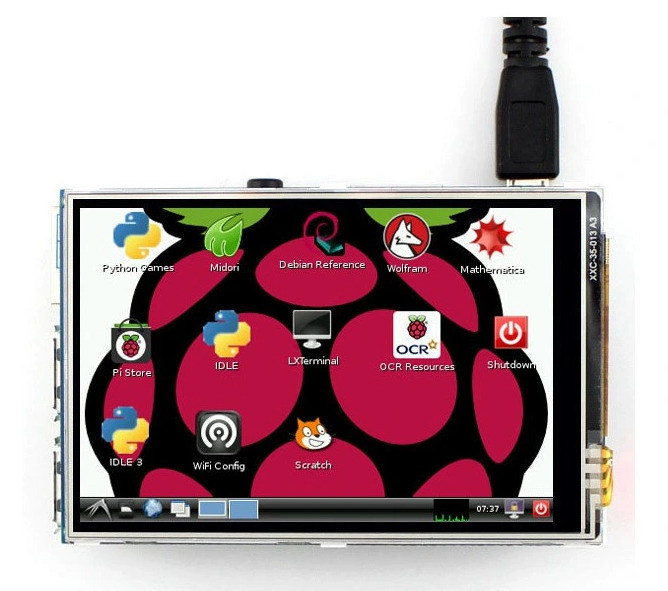
\includegraphics[width=0.8\columnwidth]{imgs/ekran.jpg}
\caption{Ekran Waveshare 9904 \cite{img_screen} \label{ekran}}
\quad
\end{figure}

Specyfikacja ekranu dotykowego Waveshare

\begin{itemize}
	\item Typ: ekran dotykowy, rezystancyjny
	\item Przekątna: 3.5"
	\item Rozdzielczość: 320px x 480px
	\item Komunikacja SPI
	\item Współpracuje z: Raspberry Pi w wersji 4B, 3B+, 3B, 2B, B+, Zero i Zero
	\item Wymiary ekranu: 85mm x 56.5mm
\end{itemize}

\subsection{Radiatory}

W celu odprowadzenia ciepła z podzespołów został zastosowany zestaw radiatorów do Raspberry Pi - z taśmą termoprzewodzącą.

Radiatory zbudowane są ze stopów metali dobrze przewodzących ciepło. Ich powierzchnia od strony zewnętrznej jest rozwinięta w postaci żeber.

\newpage
\section{Warstwa programistyczna} \label{section:warstwa_programistyczna}
\subsection{Python, jako język programowania}
% dlaczego python a nie c++
W celu realizacji funkcji prototypu zostały wzięte pod uwagę języki C++ oraz Python. Po wstępnej analizie został wybrany język Python ze względu na wsparcie producenta raspberry pi \cite{watki_jak_pisac}, większy wybór bibliotek \cite{face_detection_and_recognition_using_opencv} oraz łatwiejszy do pisania i debugowania kod \cite{face_recognition_with_python}. Jednocześnie język programowania Python charakteryzuje się wolniejszym działaniem w porównaniu do języka c++, co w moim przypadku nie jest problemem, gdyż zasobożerna biblioteka jest napisana pod pythona ale w języku c++. Dzięki czemu nie tracę na szybkości.

Z tego powodu biorąc pod uwagę przede wszystkim:
\begin{itemize}
\item większy wybór bibliotek
\item wsparcie raspberry pi
\item przejrzystość kodu
\end{itemize}
Język Python stanowi lepszy wybór z punktu widzenia działania całości projektu
\subsection{Biblioteki}
% lista bibliotek i do czego je wykorzystuje
W celu realizacji poszczególnych zadań zostały użyte następujące biblioteki języka Python:
\begin{itemize}
\item cv2, odpowiadająca za pobieranie obrazu z kamerki.
\item face\_recognition, odpowiadająca za rozpoznawanie twarzy \cite{face_recognition_github} \cite{face_recognition_implementation_on_raspberrypi} \cite{face_recognition_python}.
\item gtts, odpowiadająca za stworzenie deflautowego powitania do pliku .mp3.
\item json, odpowiadająca za zapisywanie i odczytywanie zencodowanych twarzy do plików.
\item numpy, odpowiadająca za tworzenie zoptymalizowanych pod bibliotekę rozpoznawania twarzy macierzy.
\item os, odpowiadająca za poruszanie się po folderach.
\item pygame, odpowiadająca za odtworzenie powitalnego dźwięku.
\item random, odpowiadająca za wybranie losowej ścieżki do otworzenia.
\item sys, odpowiadająca za pobranie wartości przy uruchomieniu programu sprawdzających czy zencodować wszystkich, czy tylko jedną osobę.
\item threading, odpowiadająca za wykorzystywanie przez program wszystkich dostępnych wątków procesora.
\item tkinter - odpowiada za wyświetlenie obrazu
\end{itemize}

\newpage
\subsection{Algorytm}
% prostokąty, kułka i trujkąty
Poniżej znajdują się algorytmy programów zastosowanych w projekcie:

\begin{figure}[H]%
\centering
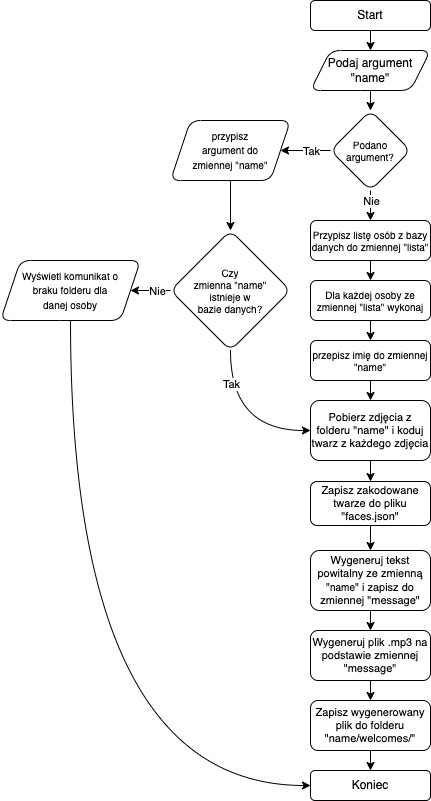
\includegraphics[width=0.7\columnwidth]{imgs/generujacy.drawio.jpg}
\caption{Program encodujący zdjęcia do plików .json \label{algorytm_encode_faces}}
\quad
\end{figure}

\begin{figure}[H]%
\centering
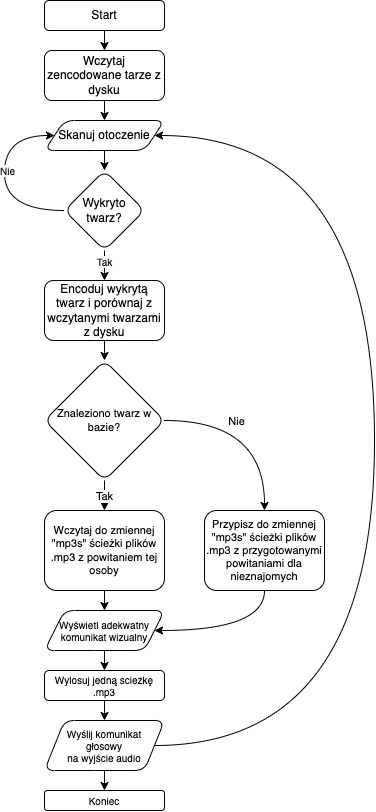
\includegraphics[width=0.7\columnwidth]{imgs/glowny.drawio.jpg}
\caption{Algorytm programu głównego \label{algorytm_start_recognition}}
\quad
\end{figure}

\subsection{Kod}
% screeny / ładne ctrl+c, ctrl+v
W tym rozdziale znajdują się listingi kodu odpowiedzialnego za realizację warstwy softwarowej projektu.
Prezentowany kod podzielony jest na następujące elementy:\newline

Zamiana obrazu twarzy na postać cyfrową (encodowanie) (Patrz \ref{listing:py_camAndStaff}).

% code
\begin{listing}[H]%
\begin{mdframed}[backgroundcolor=codebg]
\begin{minted}{python}
video_capture = cv2.VideoCapture(CAM_REF)

# Initialize some variables
face_names = []
process_this_frame = True

# start
while True:
    # Grab a single frame of video
    ret, frame = video_capture.read()
    # Resize frame of video to 1/4 size for faster face recognition
    # processing
    # small_frame = cv2.resize(frame, (0, 0), fx=0.25, fy=0.25)
    small_frame = cv2.resize(frame, (0, 0), fx=0.5, fy=0.5)
    # Convert the image from BGR color (which OpenCV uses) to 
    # RGB color (which face_recognition uses)
    rgb_small_frame = small_frame[:, :, ::-1]
    # Only process every other frame of video to save time
    thread = threading.Thread(target=encodeThisFrameFaces, 
    args=(rgb_small_frame,))
    if process_this_frame:
        # encodeThisFrameFaces(rgb_small_frame)
        print("appActiveColor: ", appActiveColor, end="\t\t")
       thread.start()
        # thread.join()
	(...)
\end{minted}
\end{mdframed}
\caption{start\_cam()}
\label{listing:py_camAndStaff}
\end{listing}

\newpage
Przypisanie rozpoznanej twarzy do zdefiniowanego w bazie danych imienia i nazwiska (Patrz \ref{listing:py_encodeThisFrameFaces_1}, \ref{listing:py_encodeThisFrameFaces_2}).
% code
\begin{listing}[H]%
\begin{mdframed}[backgroundcolor=codebg]
\begin{minted}{python}
def encodeThisFrameFaces(frame):
	timeStart = time.time()
    # Find all the faces and face encodings in the current frame of
    # video
    face_locations = face_recognition.face_locations(frame)
    face_encodings = face_recognition.face_encodings(frame, 
    face_locations)

    face_names = []
    for face_encoding in face_encodings:
        # See if the face is a match for the known face(s)
        matches = face_recognition.compare_faces(
        known_face["encodings"], face_encoding)
        name = UNKNOWN_NAME

        # Or instead, use the known face with the smallest distance
        # to the new face
        face_distances = face_recognition.face_distance(
        known_face["encodings"], face_encoding)
        best_match_index = np.argmin(face_distances)
        if matches[best_match_index]:
            name = known_face["names"][best_match_index]

        face_names.append(name)
\end{minted}
\end{mdframed}
\caption{encodeThisFrameFaces(frame) (part 1 / 2)}
\label{listing:py_encodeThisFrameFaces_1}
\end{listing}

% code
\begin{listing}[H]%
\begin{mdframed}[backgroundcolor=codebg]
\begin{minted}{python}
    # check if person desnt repeat too soon
    face_names_to_alert = []
    time_differences = {}
    for regognized_face in face_names:
        if regognized_face in ALERT_PEOPLE.keys():
            # check last seen time
            time_difference = time.time() - ALERT_PEOPLE[
            regognized_face]
            time_differences[regognized_face] = time_difference
            ALERT_PEOPLE[regognized_face] = time.time()
            if time_difference >= ALERT_DELAY_IGNORE:
                # notify
                face_names_to_alert.append(regognized_face)
                pass
            else:
                # skip
                pass
            pass
        else:
            # add to ALERT_PEOPLE
            # notify
            ALERT_PEOPLE[regognized_face] = time.time()
            face_names_to_alert.append(regognized_face)
            pass
    print(f"[{threading.active_count()}] ", *face_names_to_alert, 
    f" ({(time.time() - timeStart):.4}s)\t\t\t{time_differences}")
    
    for face in face_names_to_alert:
        say_hello(face)
    # back2idle()
    pass
\end{minted}
\end{mdframed}
\caption{encodeThisFrameFaces(frame) (part 2 / 2)}
\label{listing:py_encodeThisFrameFaces_2}
\end{listing}

\newpage
Generowanie domyślnego komunikatu głosowego  (Patrz \ref{listing:py_make_sound}).
% code
\begin{listing}[H]%
\begin{mdframed}[backgroundcolor=codebg]
\begin{minted}{python}
def create_welcome_voice_for_known_person(name, path2root=
PATH_TO_ROOT):
    person_dir_path = os.path.join(path2root, 
    KNOW_PEOPLE_DIR_PATH_NAME, name)
    welcomes_dir = os.path.join(person_dir_path, 
    WELCOMES_DIR_PATH_NAME)
    basic_welcome_file = os.path.join(welcomes_dir, 
    BASIC_WELCOME_FILE_NAME)
    create_and_save_welcome_message(f"Witaj {name}", 
    basic_welcome_file)

def create_welcome_voice_for_unknown_person(path2root=PATH_TO_ROOT):
    # create folder for unknow face
    unknowe_dir_name = f"{WELCOMES_DIR_PATH_NAME}_unknown"
    know_people_dir = os.path.join(path2root, 
    KNOW_PEOPLE_DIR_PATH_NAME)
    unknown_dir_path = os.path.join(know_people_dir, 
    unknowe_dir_name)
    if not os.path.isdir(unknown_dir_path):
        if os.path.isfile(unknown_dir_path):
            os.remove(unknown_dir_path)
        os.chdir(know_people_dir)
        os.mkdir(unknowe_dir_name)
    
    # create welocme message
    file_path = os.path.join(unknown_dir_path, 
    BASIC_WELCOME_FILE_NAME)
    create_and_save_welcome_message("Witaj nieznajomy nieznajoma", 
    file_path)
\end{minted}
\end{mdframed}
\caption{create\_welcome\_voice\_for\_[]\_person(name, path2root=PATH\_TO\_ROOT)}
\label{listing:py_make_sound}
\end{listing}

\newpage
Wysłanie komunikatu graficznego na ekran (Patrz \ref{listing:py_visual}).
% code
\begin{listing}[H]%
\begin{mdframed}[backgroundcolor=codebg]
\begin{minted}{python}
def screenVisualization():
    global appLastMode
    global lastMods2Show
    print(f"\t|{mods2ShowQueue}|")
    if len(mods2ShowQueue) > 0:
        mods2ShowQueue.sort()
        # is queue itme still valid
        if time.time() > mods2ShowQueue[0].time_end:
            # pop
            mods2ShowQueue.pop(0)
            screenVisualization()
            pass
        else:
            activeMode2show = mods2ShowQueue[0]
            # change only if mod2show is new
            if activeMode2show != lastMods2Show:
                Tk.configure(background=appBackground[
                activeMode2show.activeMode])
                Tk.update()
                lastMods2Show = activeMode2show
                appLastMode = activeMode2show.activeMode;
                pass
            pass
        pass
    else:
        # change to idle (expect it is not idle)
        if appLastMode != Mods.IDLE:
            Tk.configure(background=appBackground[Mods.IDLE])
            Tk.update()
        appLastMode = Mods.IDLE;
\end{minted}
\end{mdframed}
\caption{screenVisualization()}
\label{listing:py_visual}
\end{listing}

\newpage
Wysłanie komunikatu głosowego do głośników  (Patrz \ref{listing:py_play_sound}).
% code
\begin{listing}[H]%
\begin{mdframed}[backgroundcolor=codebg]
\begin{minted}{python}
def say_hello(name, path2root=PATH_TO_ROOT):
    global appActiveMode
    global appActiveName
    
    appActiveName = name
    
    if name == "Unknown":
        appActiveMode = Mods.UNKNOWN
        pass
    else:
        appActiveMode = Mods.KNOWN
        path_to_welcomes_for_name = os.path.join(path2root,
        KNOW_PEOPLE_DIR_PATH_NAME, name, WELCOMES_DIR_PATH_NAME)
        
        # get mp3's
        mp3s = []
        for file in os.listdir(path_to_welcomes_for_name):
            print(file)
            extension = os.path.splitext(file)[1] # extension of file
            print(extension)
            if extension.lower() == ".mp3":
                mp3s.append(os.path.join(path_to_welcomes_for_name, 
                file))
        print(mp3s)        
        
        # rand file to play
        mp3_to_paly = random.choice(mp3s)
        print(mp3_to_paly)
        
        # play      
        pygame.mixer.init()
        pygame.mixer.music.load(mp3_to_paly)
        pygame.mixer.music.play()
        while pygame.mixer.get_busy() == True:
            continue
        # back2idle()
    pass
\end{minted}
\end{mdframed}
\caption{say\_hello(name, path2root=PATH\_TO\_ROOT)}
\label{listing:py_play_sound}
\end{listing}

\newpage
Obsługa sytuacji w zależności od tego czy twarz została rozpoznana  (Patrz \ref{listing:py_sytuacje}).
% code
\begin{listing}[H]%
\begin{mdframed}[backgroundcolor=codebg]
\begin{minted}{python}
def say_hello(name, path2root=PATH_TO_ROOT):
    global addPersoneMode2queue
    
    appActiveName = name
    
    # get mp3' dir
    mp3s = []
    path_to_welcomes_for_name = os.path.join(path2root, 
    KNOW_PEOPLE_DIR_PATH_NAME)
    if name == "Unknown":
        addPersoneMode2queue(Mods.UNKNOWN)
        path_to_welcomes_for_name = os.path.join(
        path_to_welcomes_for_name, "welcomes_unknown")
    else:
        addPersoneMode2queue(Mods.KNOWN, name)
        path_to_welcomes_for_name = os.path.join(
        path_to_welcomes_for_name, name, WELCOMES_DIR_PATH_NAME)
        
    # get mp3s
    for file in os.listdir(path_to_welcomes_for_name):
        print(file)
        extension = os.path.splitext(file)[1] # extension of file
        print(extension)
        if extension.lower() == ".mp3":
            mp3s.append(os.path.join(path_to_welcomes_for_name, 
            file))
    print(mp3s)        
        
    # rand file to play
    mp3_to_paly = random.choice(mp3s)
    print(mp3_to_paly)
    
    # play      
    pygame.mixer.init()
    pygame.mixer.music.load(mp3_to_paly)
    pygame.mixer.music.play()
    while pygame.mixer.get_busy() == True:
        continue
\end{minted}
\end{mdframed}
\caption{say\_hello(name, path2root=PATH\_TO\_ROOT)}
\label{listing:py_sytuacje}
\end{listing}

\newpage
\section{Warstwa produktowa} \label{section:warstwa_produkcyjna} % wysłać skreeny z solidworksa i zdjęcia obudowy
Prototyp to nie tylko elektronika oraz oprogramowanie. Bardzo ważnym elementem jest stworzenie całościowego produktu, do czego niezbędne jest zaprojektowanie oraz wykonanie odpowiedniej obudowy. W celu realizacji tego zadania zostały użyte poniższe programy:
\begin{itemize}
\item SOLIDWORKS – do tworzenia projektu obudowy
\item ultimaker cura – do przygodowania wexportowanego z solidworksa pliku do postaci g-code którą czytają drukatki 3D.
\item octoprint (+ Raspbarry pi) – do nadzorowania wydruku
\end{itemize}
oraz prototypowanie przy pomocy drukarki 3D.
\subsection{Technologia druku 3D}
Druk 3D został wynaleziony z konieczności szybkiego i stosunkowo taniego przygotowywania wszelkiego rodzaju prototypów praktycznie we wszystkich branżach działalności gospodarczej. 
Obecnie prototypowanie przy użyciu wydruków 3D zdecydowanie ułatwia i przyspiesza całość prac od projektu do wykonania wyrobu końcowego.

Zalety prototypowania przy pomocy druku 3D \cite{prototyp3dzalety}
\begin{itemize}
\item Łatwość modyfikacji projektu 
\item Możliwość natychmiastowego rozpoczęcia drukowania projektu
\item Brak konieczności oczekiwania na realizację zadania przez firmy zewnętrzne
\item Możliwość zastosowania materiałów o różnych własnościach
\item Relatywnie mała cena
\end{itemize}

Drukarki 3D używane do prototypowania, wykorzystują 2 podstawowe technologie przyrostowe.
\cite{prototyp3dzalety}
\begin{itemize}
\item SLA, oraz
\item FDM
\end{itemize}
\textbf{W technologii SLA} do wydruku wykorzystuje się żywicę, która jest materiałem światło utwardzalnym. Poszczególne warstwy nanosi się na specjalnie zaprojektowanej płytce. Poszczególne warstwy utwardzane są wiązką laserową. \cite{jakie_materialy_w_druku}

Zaletą tej metody jest duża dokładność otrzymanego modelu, natomiast podstawową wadą tej technologii jest:
\begin{itemize}
\item stosunkowo wysoki koszt użycia w warunkach domowych oraz
\item konieczność stosowania wyciągów mechanicznych w celu odprowadzenia powstających w trakcie procesu oparów.
\end{itemize}

\textbf{W technologii FDM} drukarki do druku korzystają z tworzyw plastikowych takich jak ABS oraz PLA \cite{jak_wybrac_tworzywo_do_drukarek} \cite{jakie_materialy_w_druku}.

Do celów realizacji niniejszego projektu wybrałem metodę FDM ze względu na jej niewielki koszt oraz już posiadaną drukarkę 3D wykorzystującą właśnie tą technologię druku. 
Do druku drukarki wykorzystujące technologię FDM korzystają z tworzyw plastikowych takich jak ABS oraz PLA.
Filament, czyli materiał drukujący ("Tusz"), przechodzi przez głowicę drukarki, gdzie następuje jego podgrzanie aż do uzyskania formy płynnej materiału. 
Następnie jest on wyciskany przez dedykowaną dyszę (stosowane są różne średnice dysz) na stół roboczy. 
Dysza rozprowadza w przestrzeni roboczej filament w postaci nakładania na siebie kolejnych warstw, zgodnie z przygotowanym wcześniej projektem. 
Po nałożeniu warstwy następuje jej schłodzenie i filament twardnieje. 
Po naniesieniu ostatniej warstwy wydruku, wydruk (i elementy drugarki) musi się schłodzić, a następnie sam schodzi z powierzchni drukującej.

Zgodnie z \cite{prototyp3dzalety} „(...) prototypowanie z wykorzystaniem druku 3D pozwala na wypracowanie oszczędności – czasu i pieniędzy. Umożliwia szybkie testowanie prototypów i przyspiesza czas, jaki niezbędny jest do wprowadzenia docelowego produktu na rynek. Dodatkowo na każdym etapie procesu prototypowania można otrzymać natychmiast podgląd wydruku i śledzić proces powstawania modelu (...)”

\begin{figure}[H]%
\centering
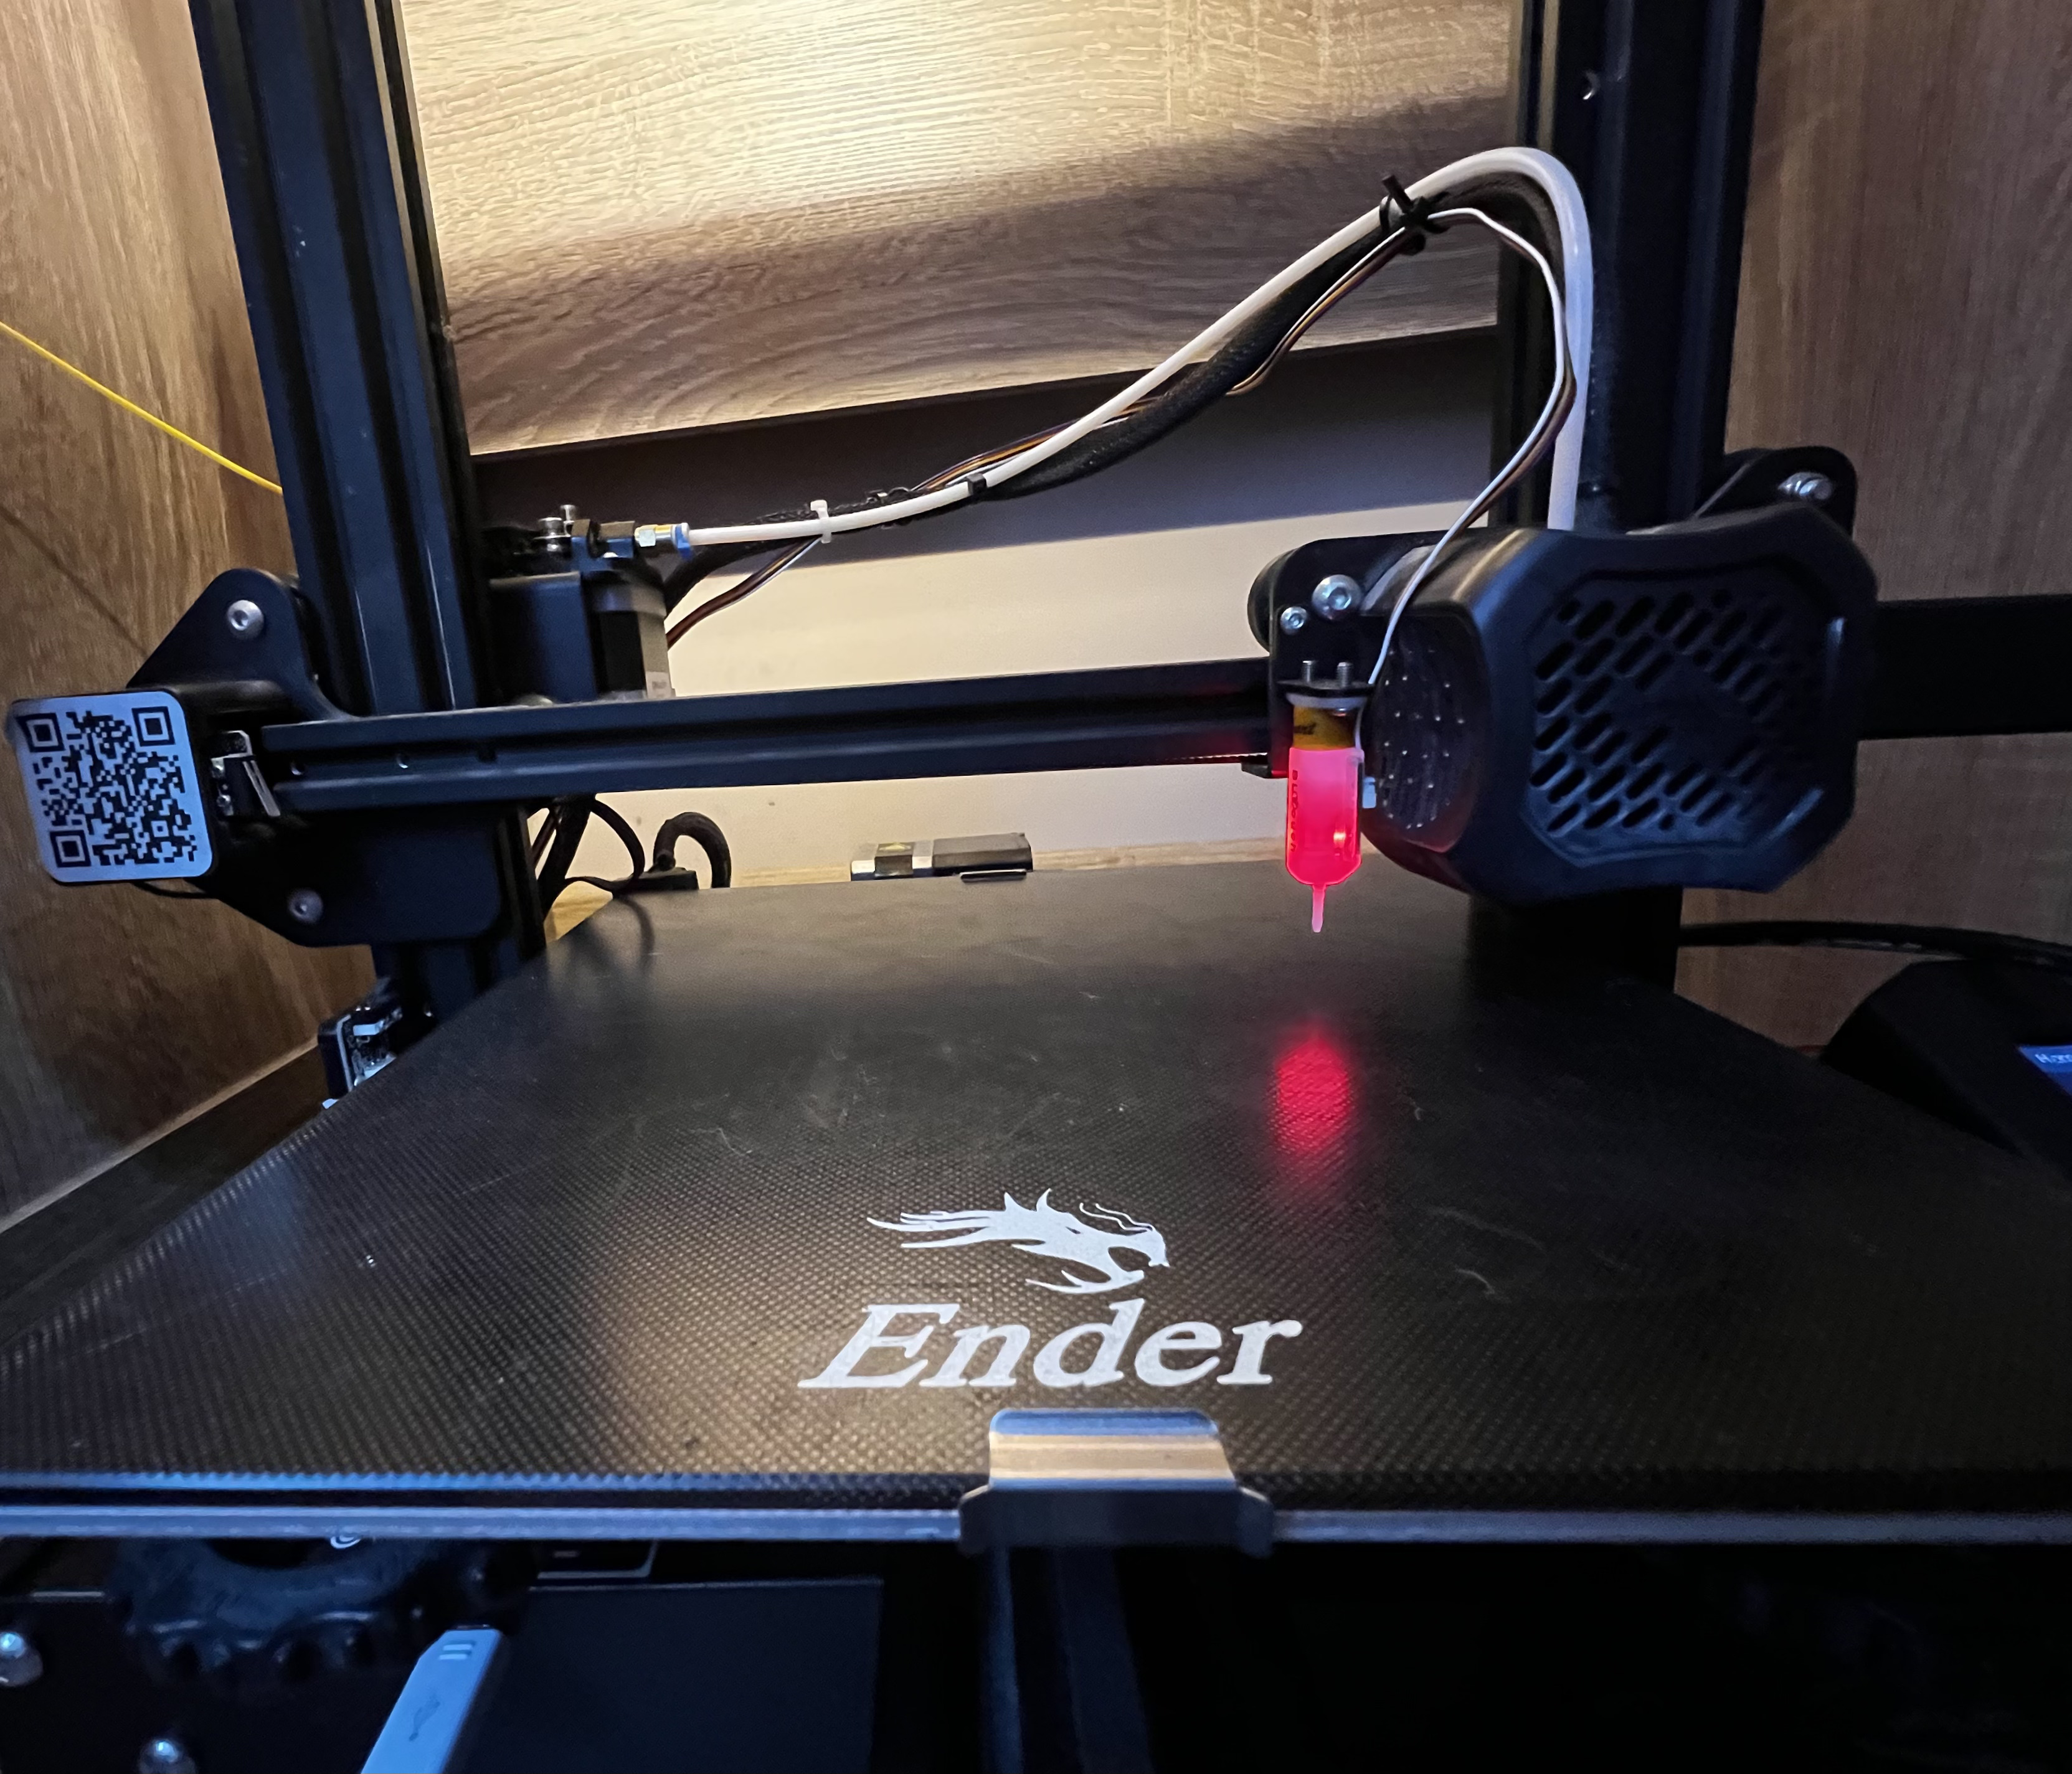
\includegraphics[width=0.8\columnwidth]{imgs/ender3v2.jpg}
\caption{Drukarka 3D Creality Ender wykorzystana w projekcie \label{ender3d}}
\quad
\end{figure}

\subsection{Projekt obudowy}
W celu wykonania projektu obudowy zostały wykorzystane oprogramowanie solidworks	 w wersji 21
W początkowej fazie użyto oprogramowania autodesk fusion 360, jednak nie mogłem znaleźć w nim wielu narzędzi których się nauczyłem korzystać w solidworksie

W ramach wykonania projektu ostatecznego były wprowadzane poprawki do projektu zgodnie z zasadą PDCA stanowiącą podstawę zwinnego projektowania \newline
\textbf{P – PLAN}: zaplanuj \newline
\textbf{D – DO}: wykonaj \newline
\textbf{C – CHECK}: sprawdź \newline
\textbf{A – ACT}: popraw

\subsection{Wykonanie obudowy}
W celu osiągnięcia ostatecznego wyniku przeprowadzono kilka iteracji cyklu Deminga (PDCA) \cite{leanByJK}. W tym celu dokonywano także poprawek ustawień drukarki.

\begin{figure}[H]%
\centering
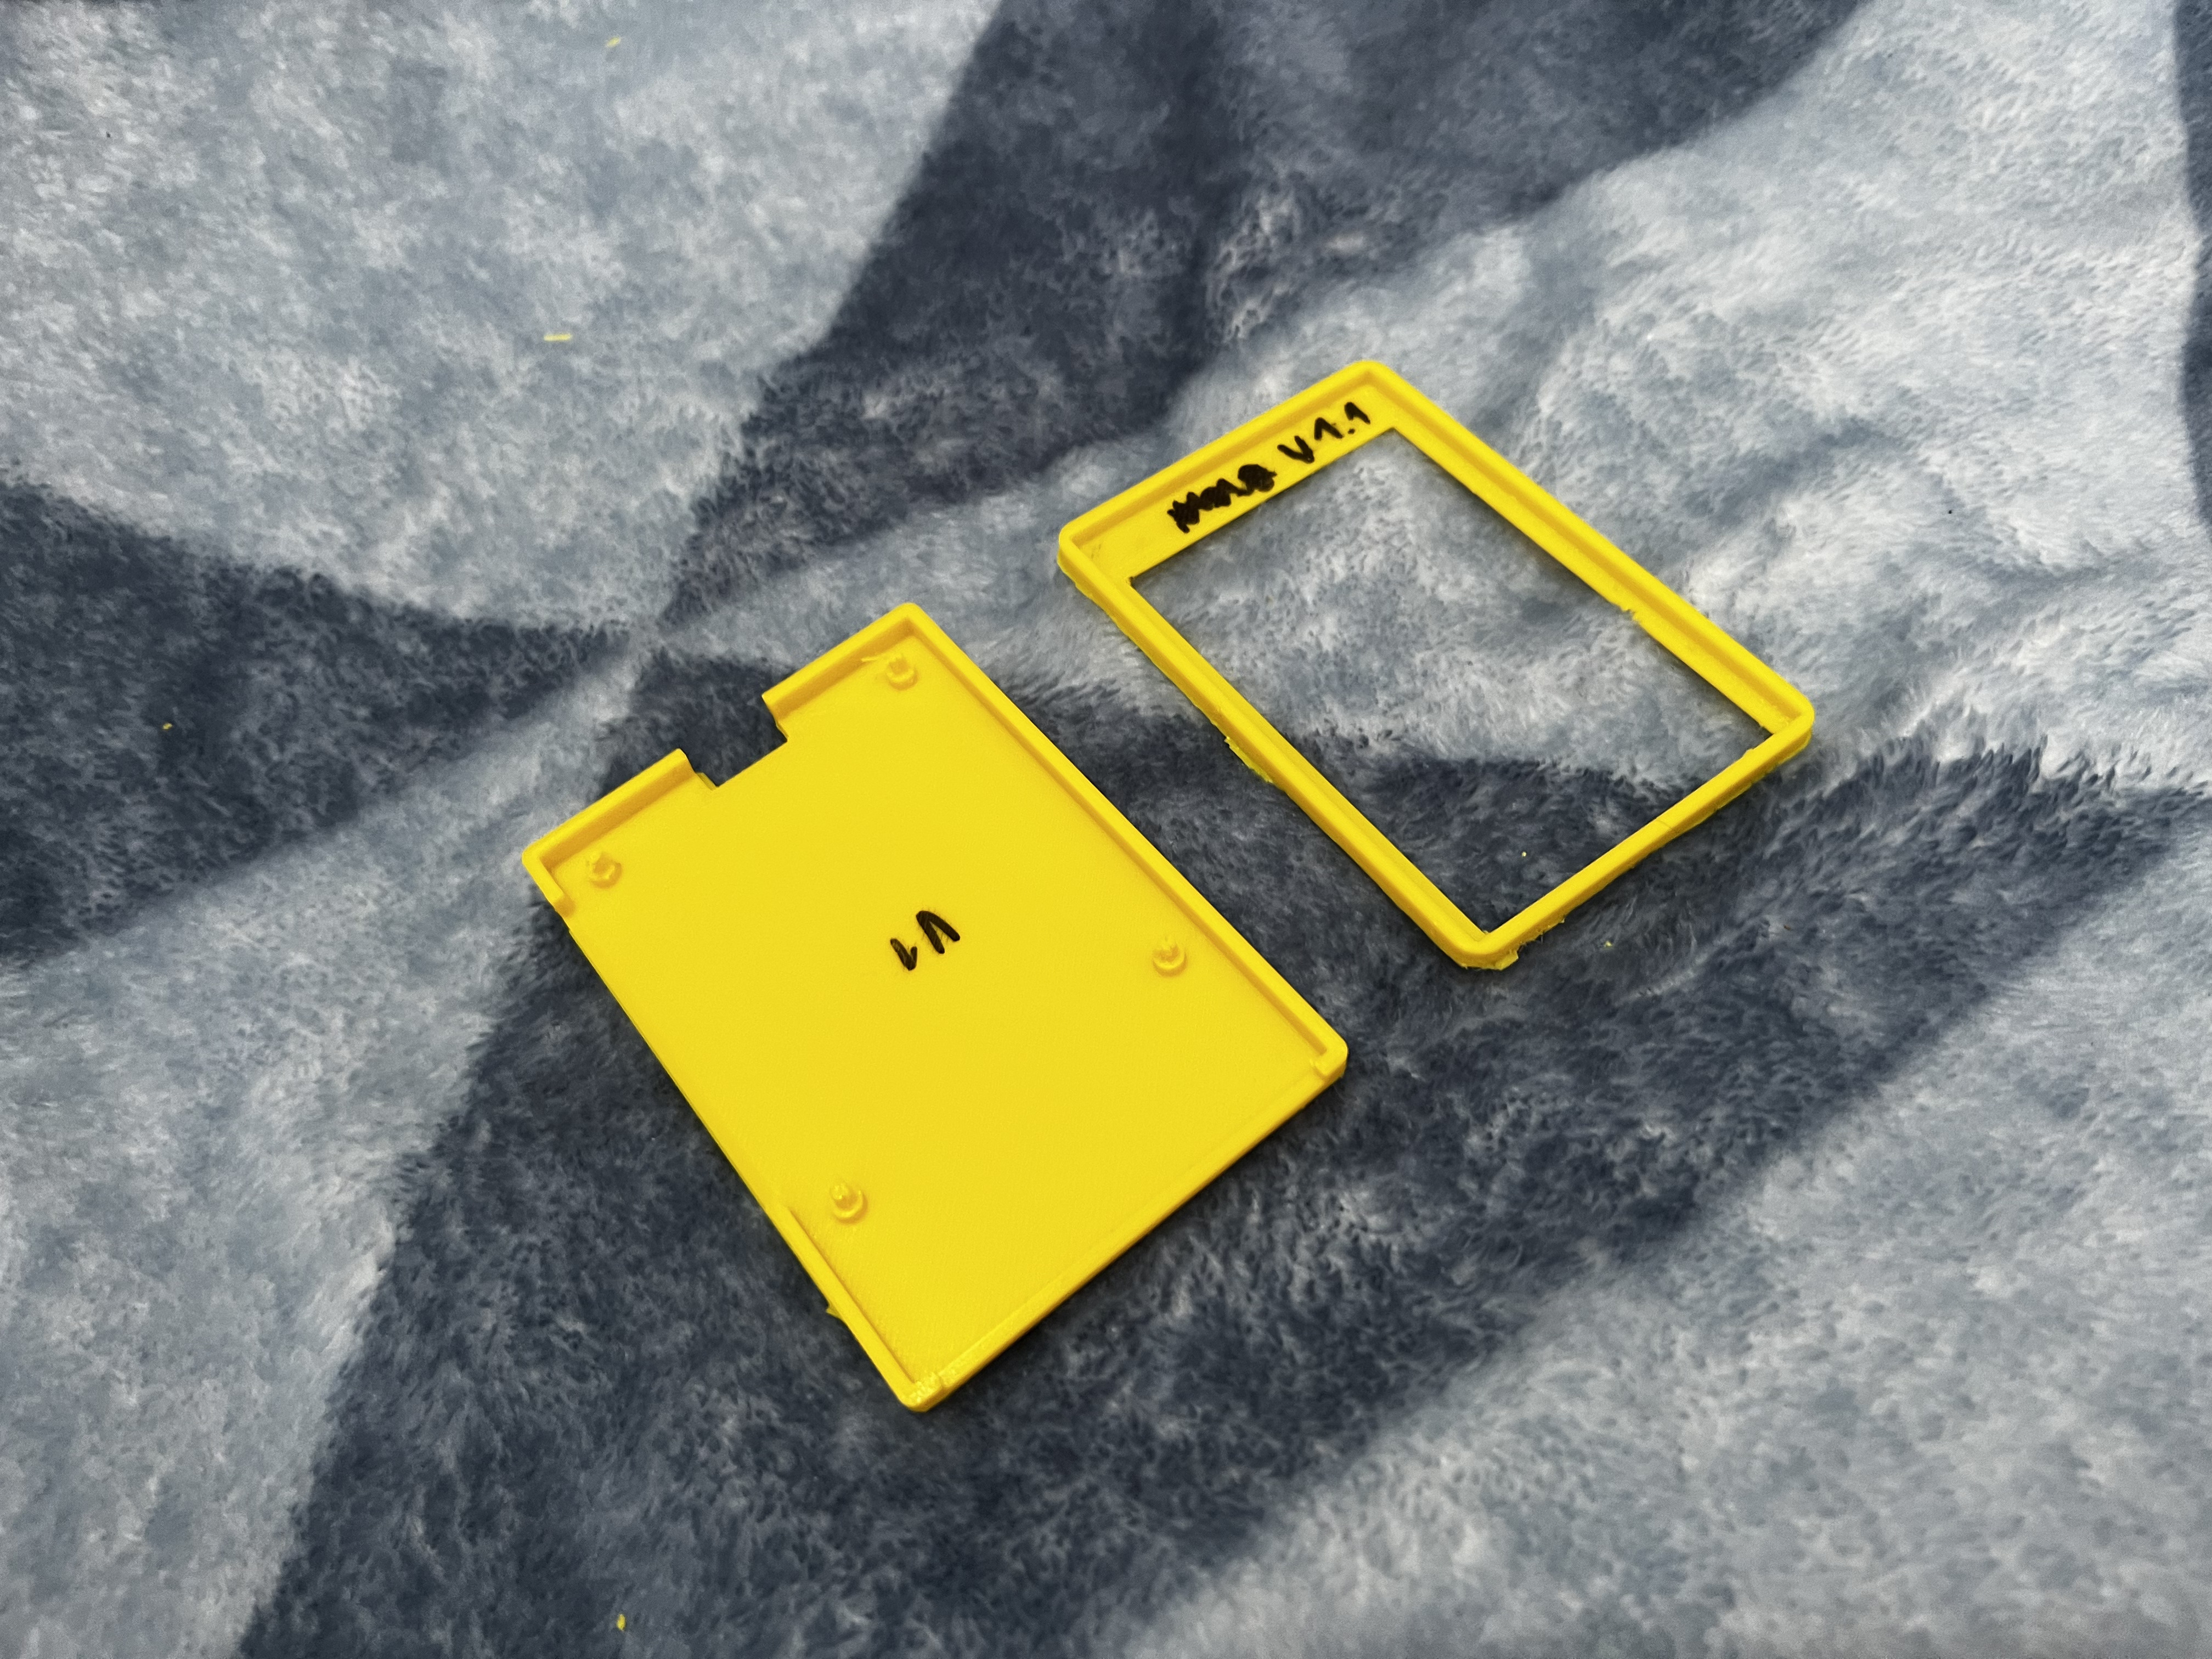
\includegraphics[width=0.8\columnwidth]{imgs/print_0.jpg}
\caption{Iteracja Początkowa \label{PDCA_00}}
\quad
\end{figure}

W pierwszej iteracji (Patrz rys. \ref{PDCA_00}) okazało się, że wymiary i rozmieszczenie bolców jest lekko przesunięte względem Raspberry Pi

\newpage
W jednej z pośrednich iteracji (Patrz rys. \ref{PDCA_01}) okazało się, że wymiary i rozmieszczenie bolców jest lekko przesunięte względem Raspberry Pi

\begin{figure}[H]%
\centering
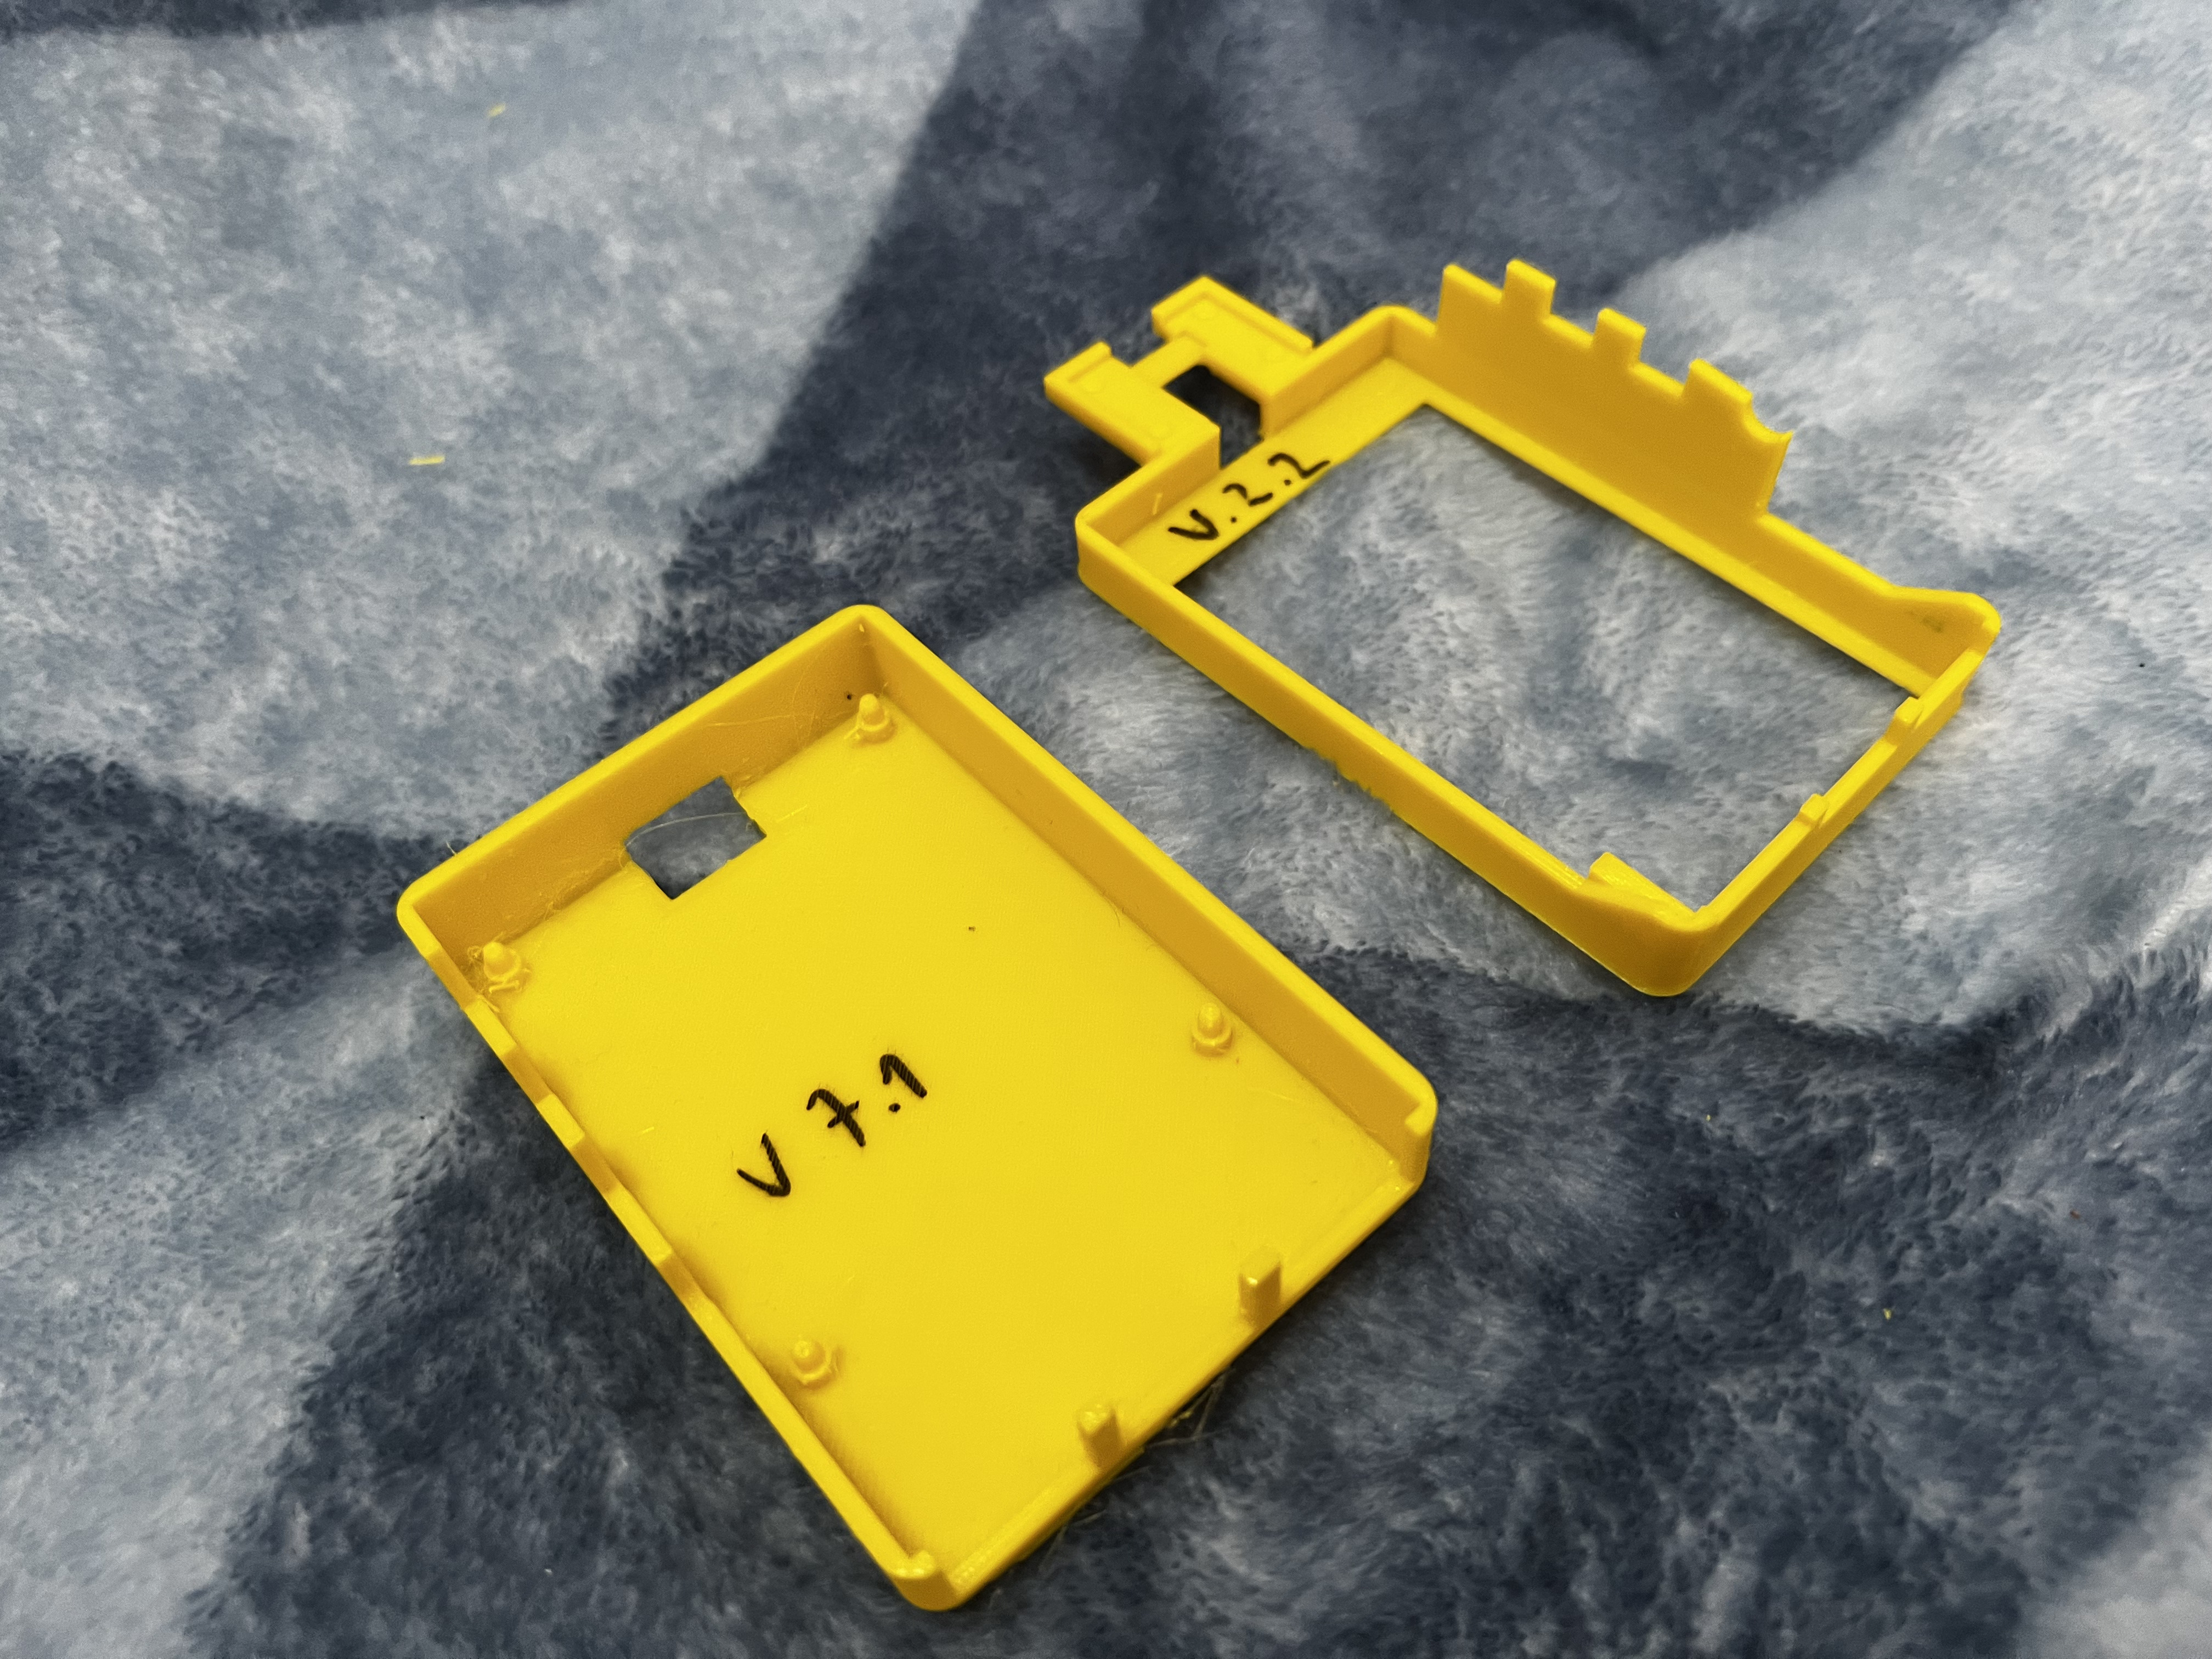
\includegraphics[width=0.8\columnwidth]{imgs/print_1.jpg}
\caption{Iteracja pośrednia 1 \label{PDCA_01}}
\quad
\end{figure}

\begin{figure}[H]%
\centering
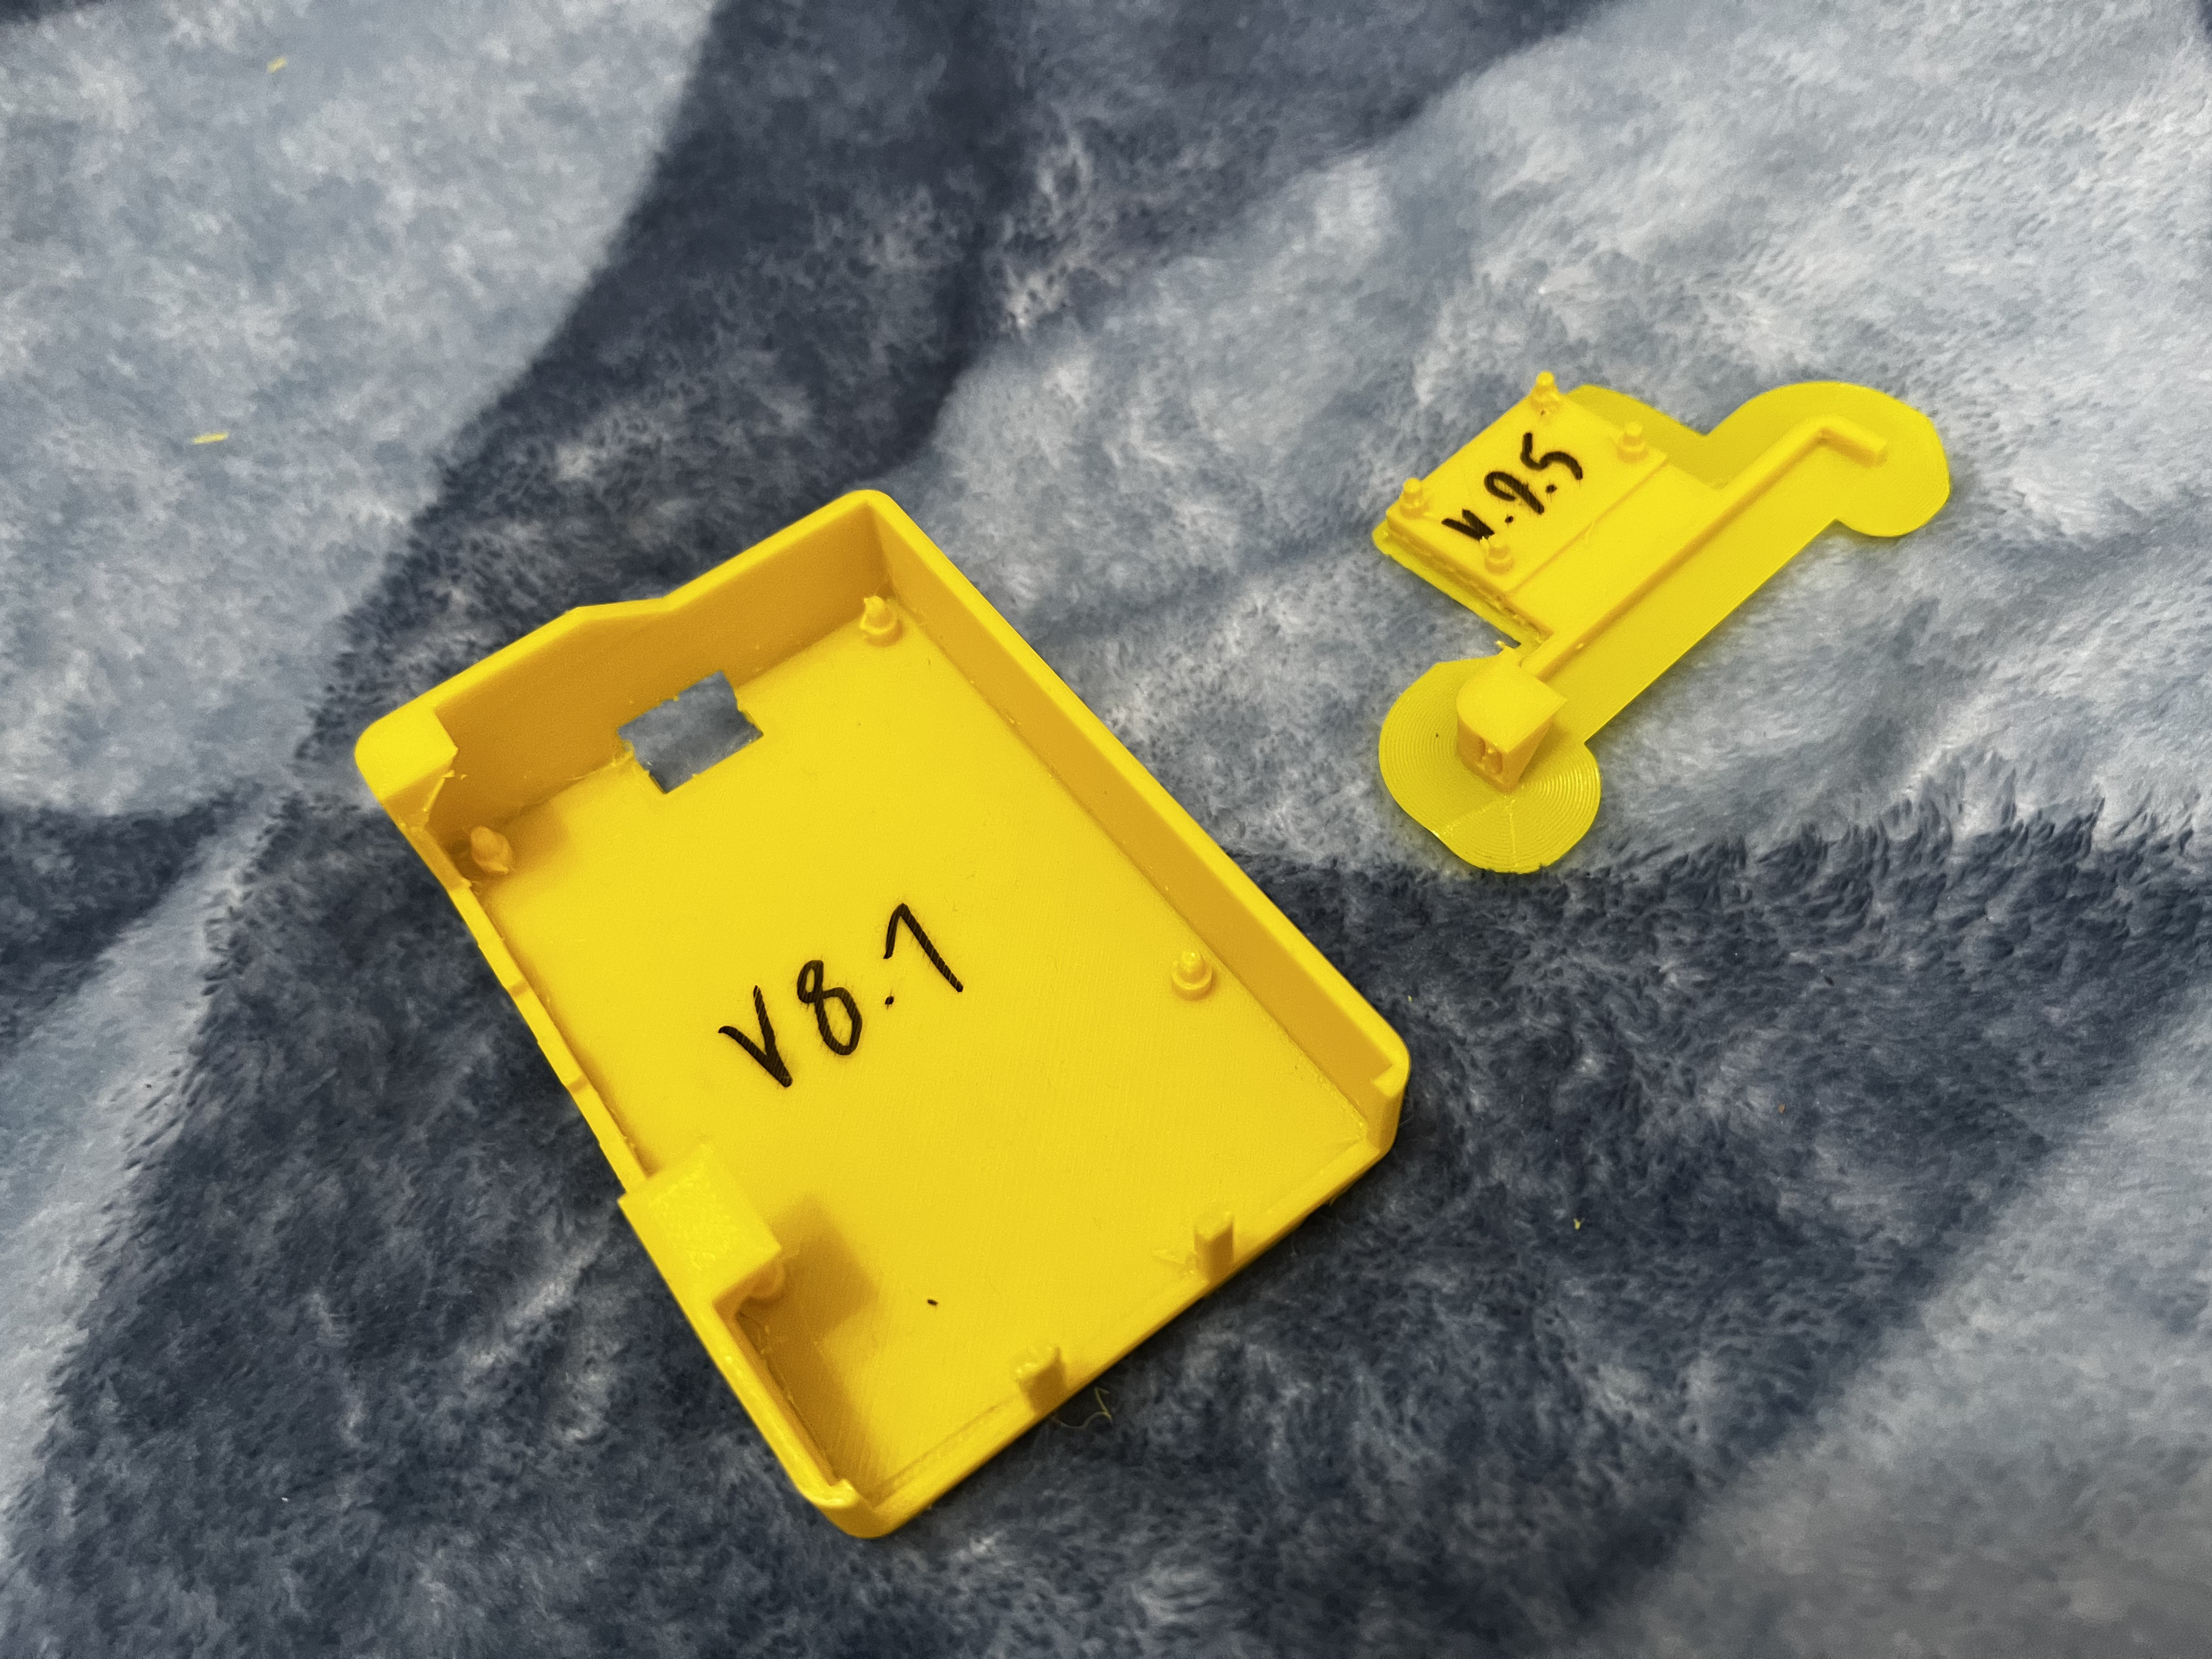
\includegraphics[width=0.8\columnwidth]{imgs/print_2.jpg}
\caption{Iteracja pośrednia 2 \label{PDCA_02}}
\quad
\end{figure}

Następna iteracji (Patrz rys. \ref{PDCA_02}) miała na celu wydrukowanie poprawynch wymiarów dla kamery. Z powodu niewielkich rozmiarów urządzenia nie było łatwo dokładnie zmierzyć otworów. Nawet z uwzględnieniem niepewności pomiarowej trzeba było wydrukować komponent kilka razy z różnicą kilku dziesiątych mm.

\begin{figure}[H]%
\centering
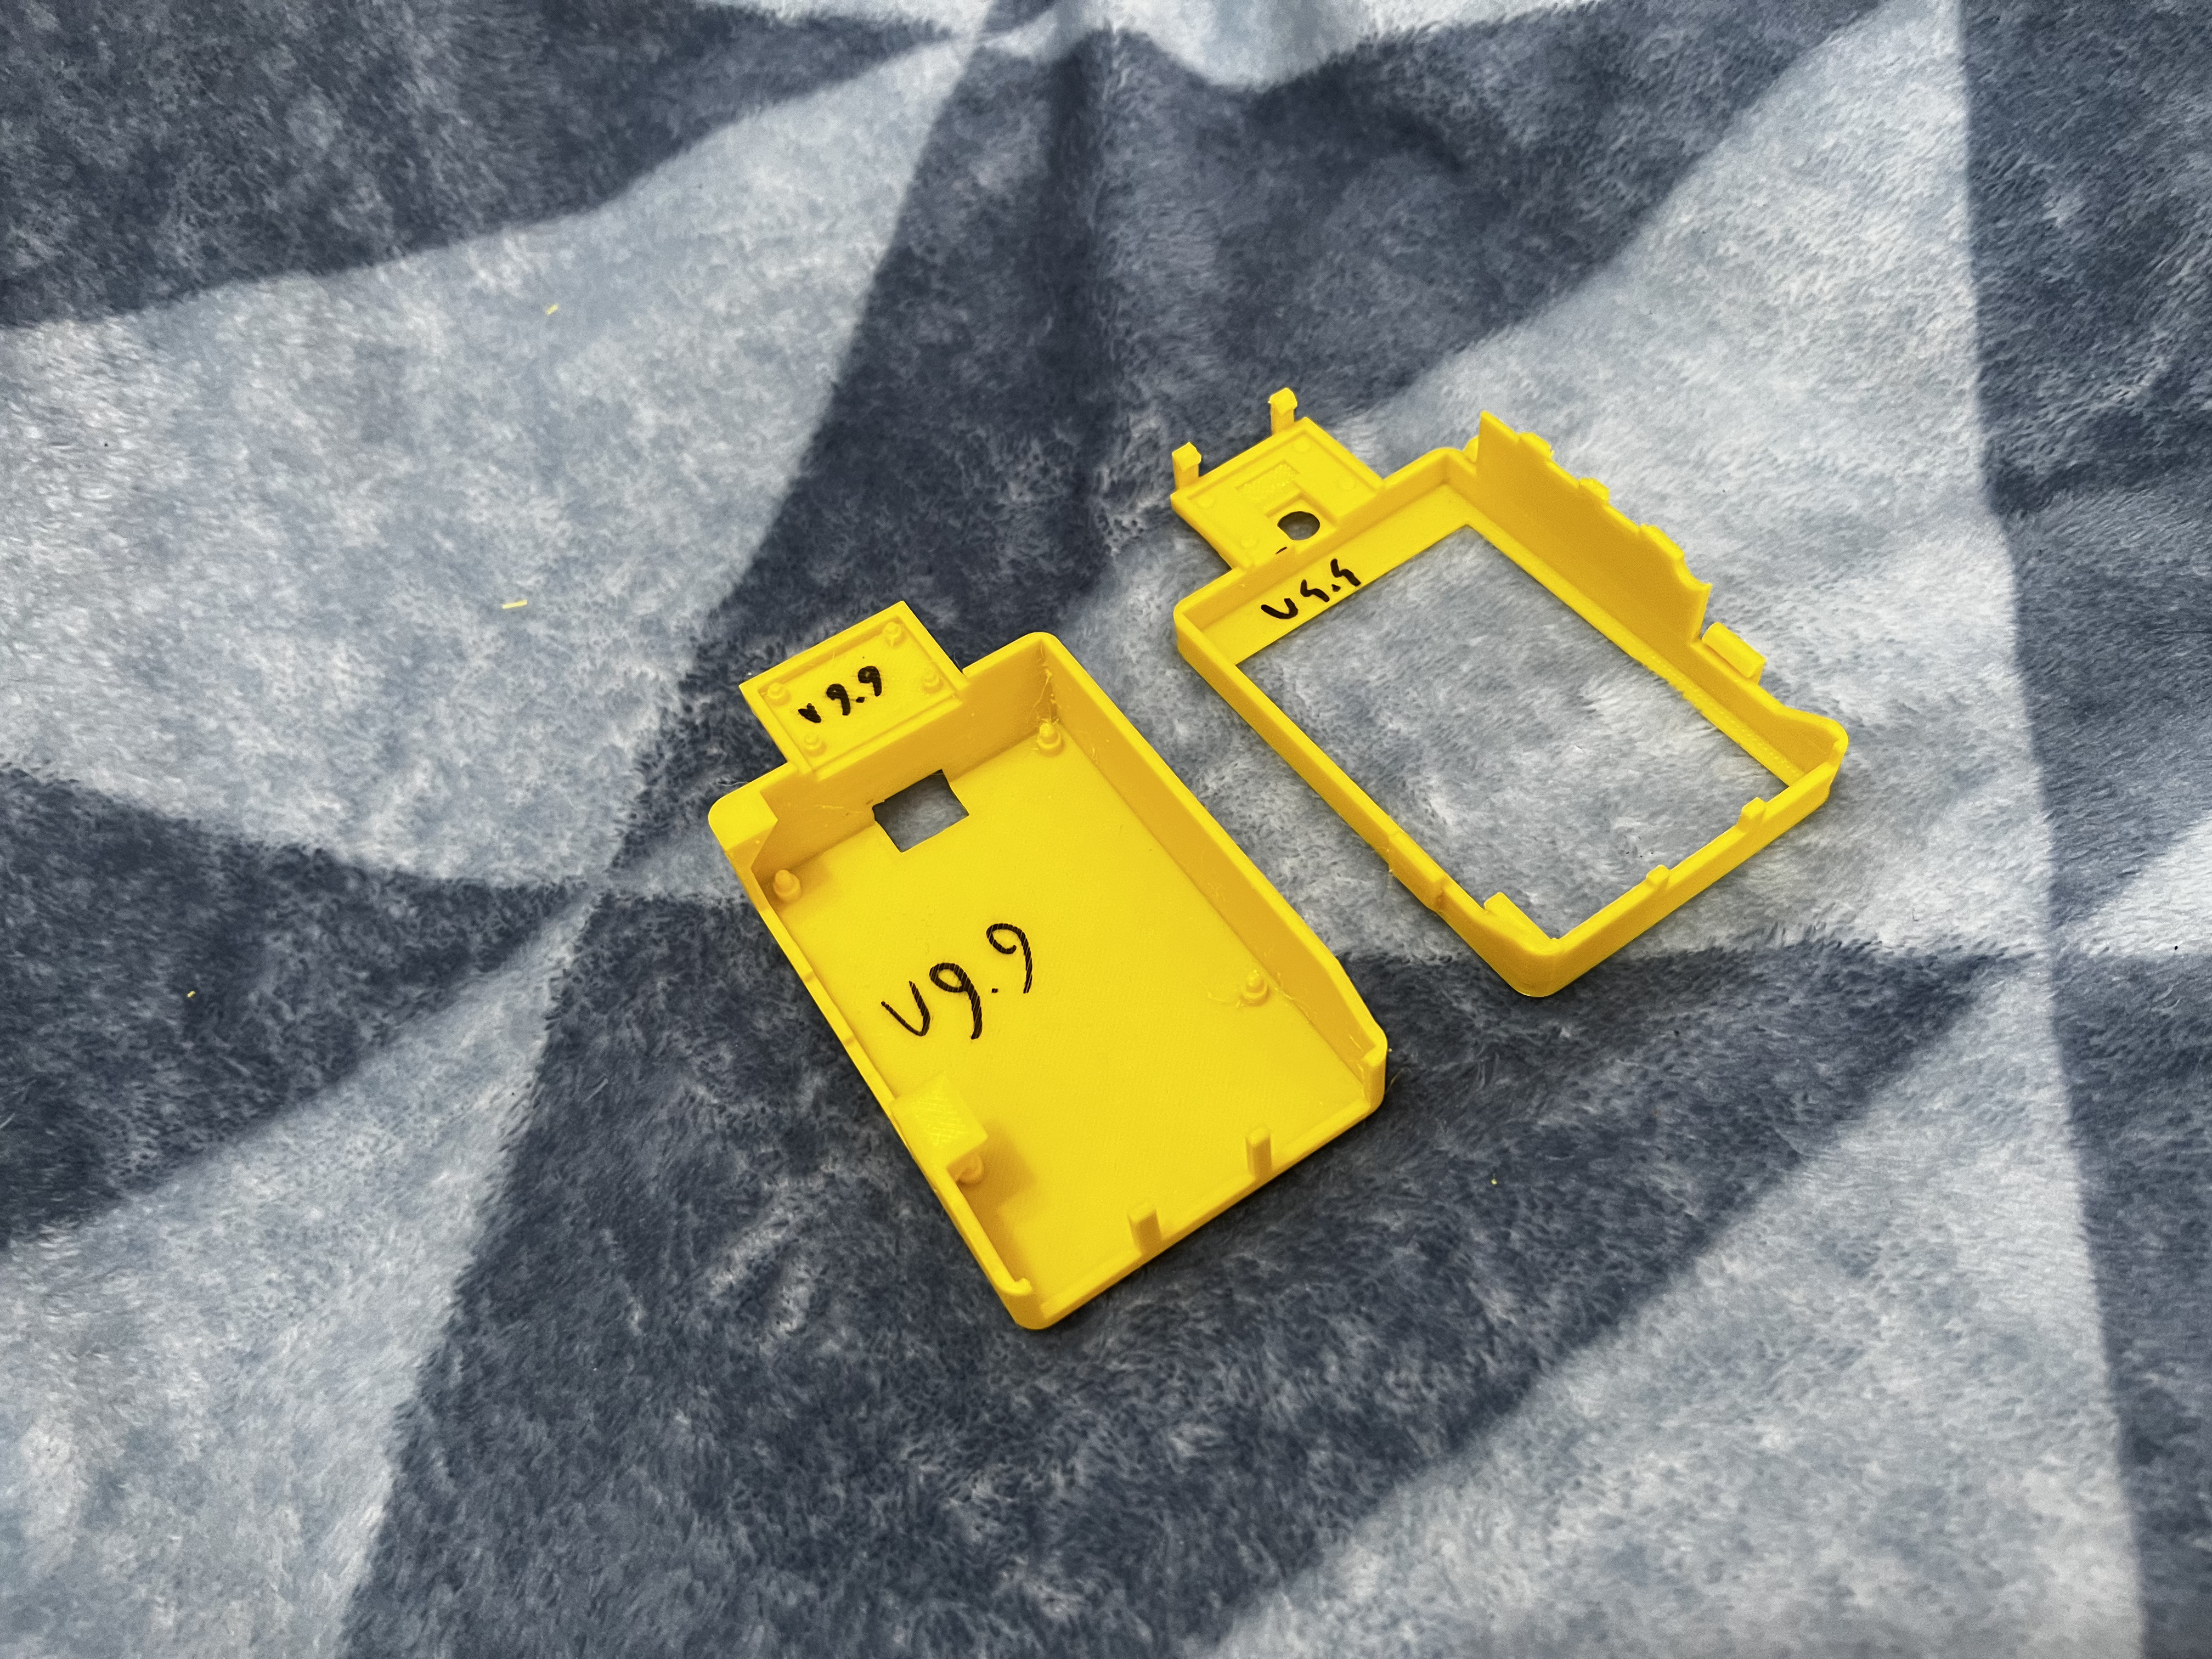
\includegraphics[width=0.8\columnwidth]{imgs/print_3.jpg}
\caption{Iteracja pośrednia 3 \label{PDCA_03}}
\quad
\end{figure}

W jednej z końcowych iteracji (Patrz rys. \ref{PDCA_03}) celem było wpasowanie obu części obudowy w siebie nawzajem. Na "Papierze" wszystkie wymiary się zgadzały i powinny pasować. Jednak z względu niedoskonałości wydruku było inaczej.

\newpage
Ostatnia iteracjia (Patrz rys. \ref{PDCA_END}) złożona z zamontowanymi w niej częściami, oraz śrubą aparatową pod stojak.
\begin{figure}[H]%
\centering
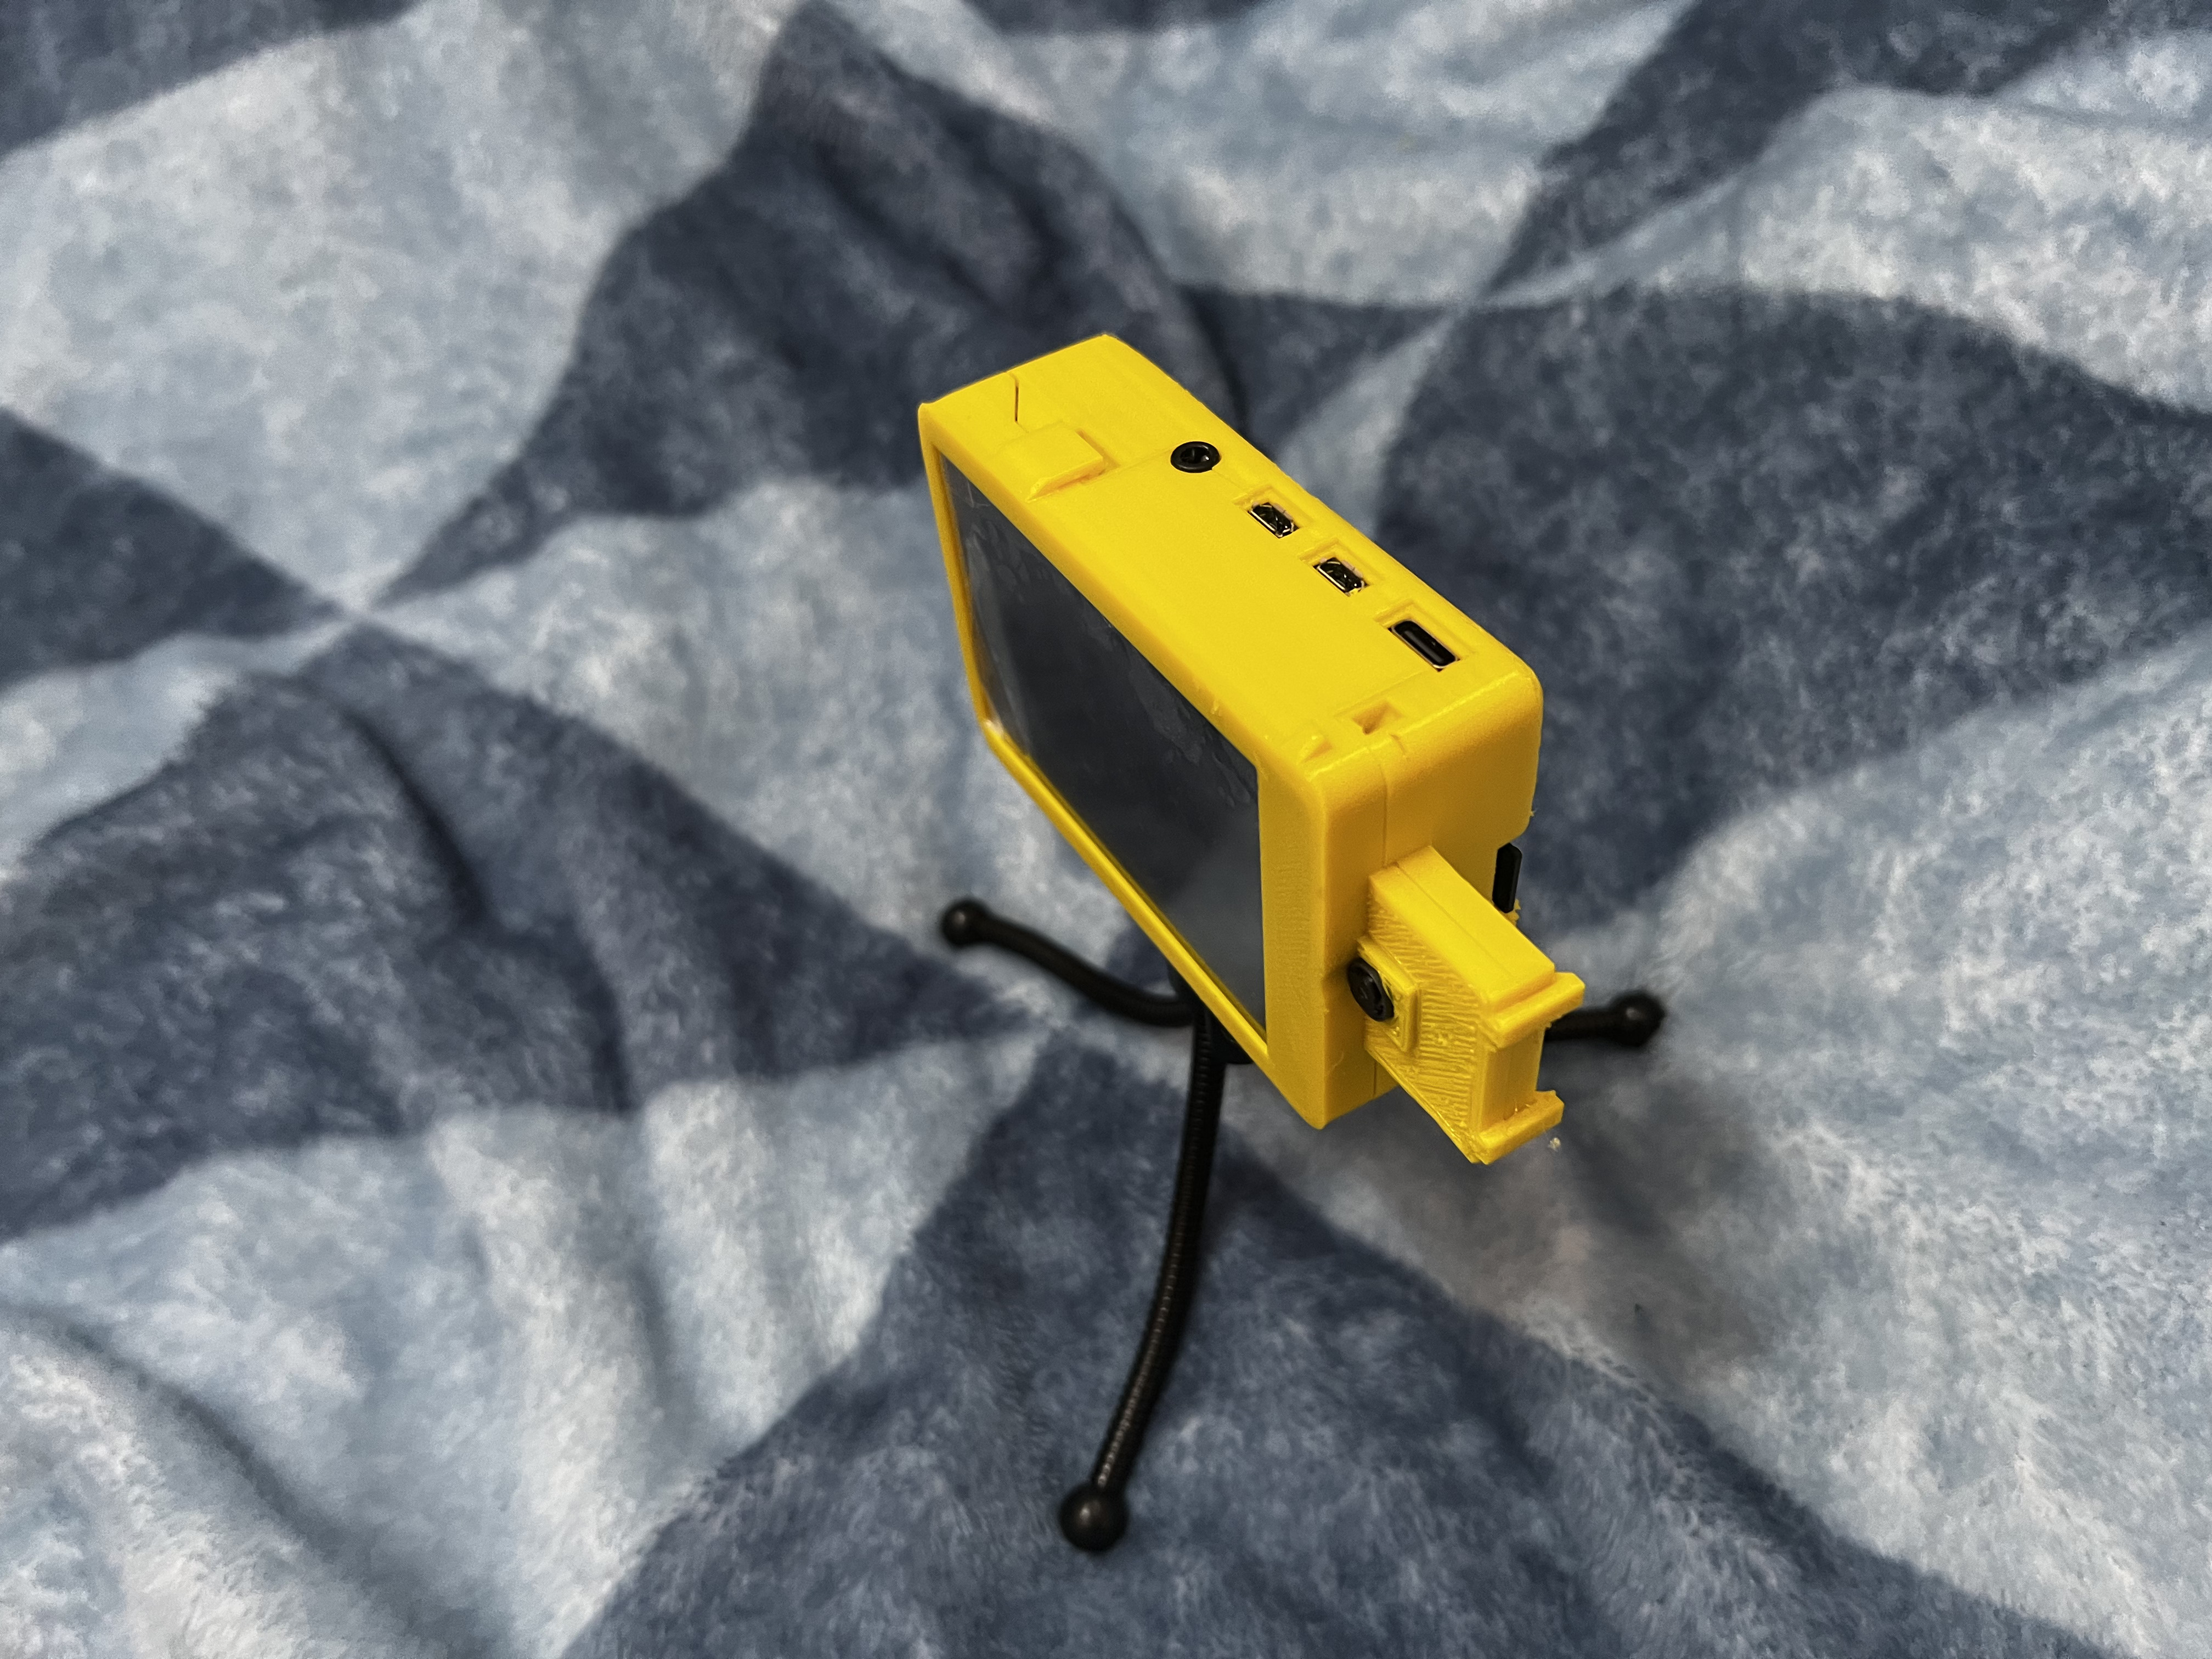
\includegraphics[width=0.8\columnwidth]{imgs/print_last_assembled.jpg}
\caption{Iteracja końcowa \label{PDCA_END}}
\quad
\end{figure}

Wszystkie wydrukowane Iteracje PDCA (Patrz rys. \ref{PDCA_ALL}).

\begin{figure}[H]%
\centering
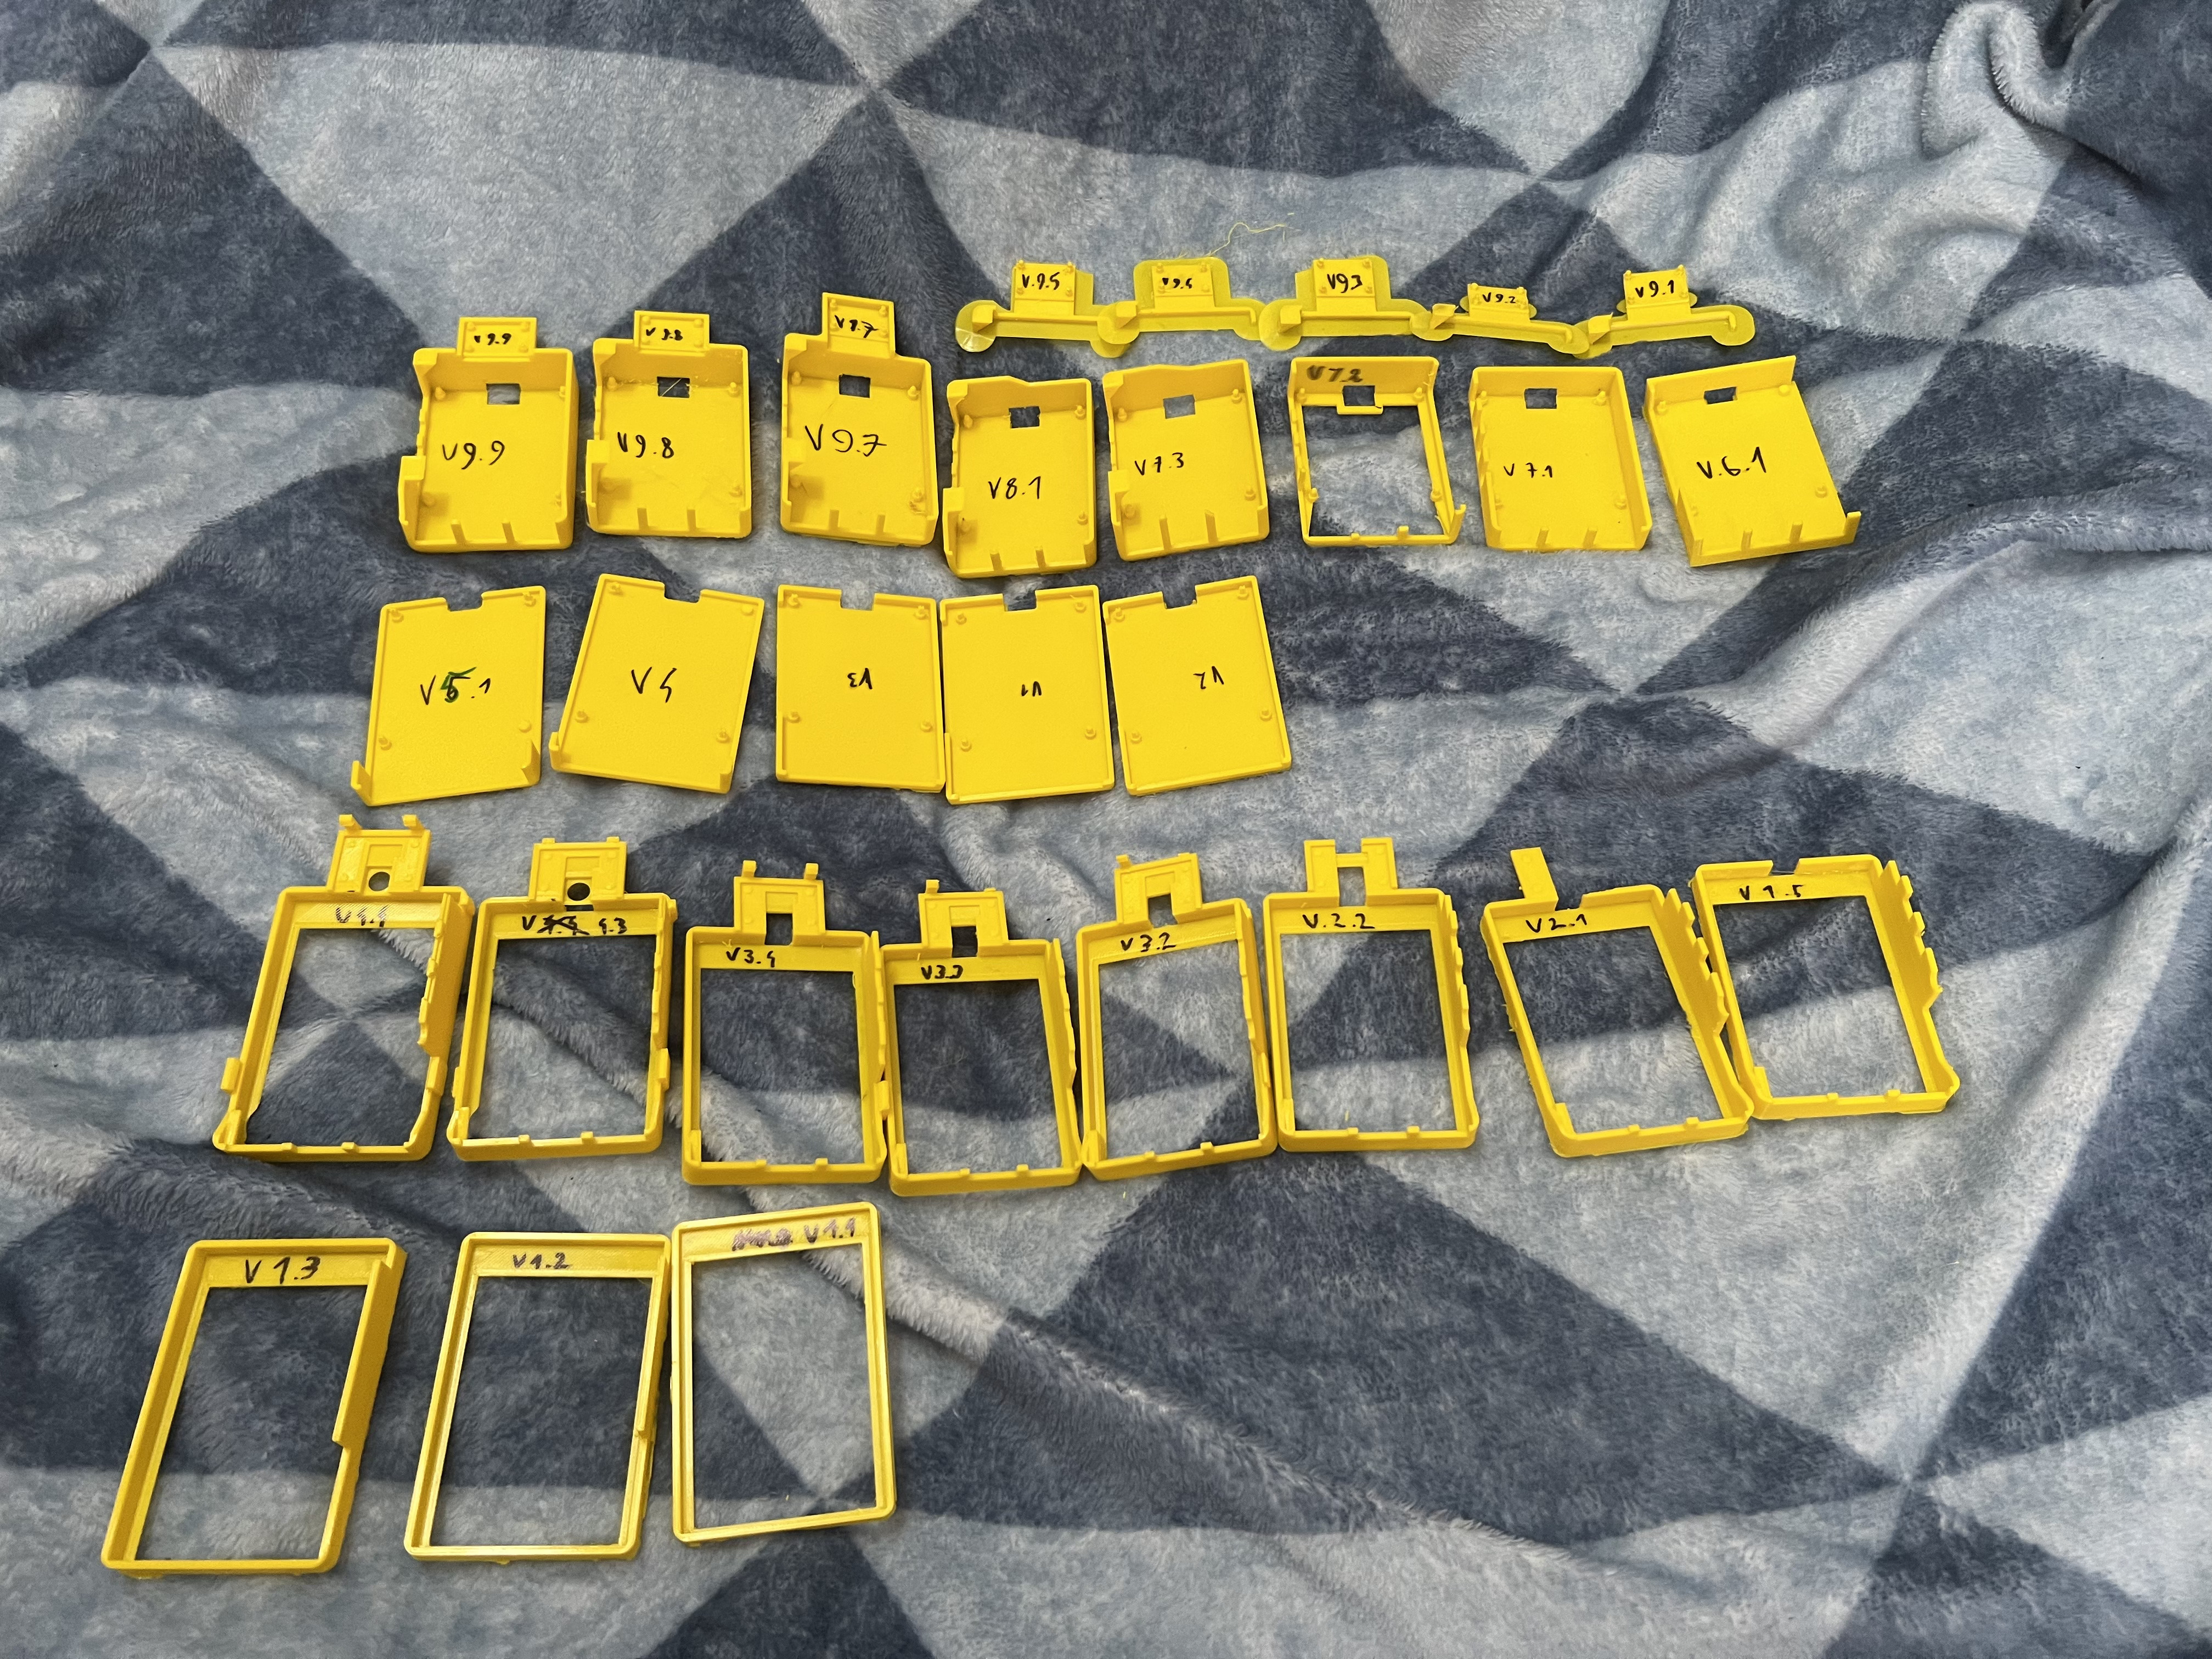
\includegraphics[width=0.8\columnwidth]{imgs/print_all.jpg}
\caption{Wszystkie wydrukowane Iteracje \label{PDCA_ALL}}
\quad
\end{figure}

\section{Realizacja projektu} \label{section:realizacja}
\subsection{Napotkane problemy}
W trakcie realizacji projektu napotkano następujące problemy.
\begin{itemize}
	\item \textbf{Wykorzystanie tylko jednego rdzenia procesora} (wątku). Raspberry Pi wyposażony jest w procesor czterordzeniowym, dzięki czemu można jednocześnie realizować 4 równoległe operacje. \newline \textbf{Problem:} \newline Okazało się że procesor Raspberry ma problemy z wykorzystaniem większej lioczby wątków w ramach jednego programu. \newline \textbf{Rozwiązanie:} \newline Użyto biblioteki threading do pracy na wątkach.
	\item \textbf{Brak możliwość realizacji komunikatów głosowych.} \newline \textbf{Problem:} \newline Pierwotnie zastosowany głośnik nie posiadał wsparcia dla realizacji komunikatów głosowych zapisanych w pamięci prototypu. Jedyną możliwością było odtwarzanie plików przez Spotify. \newline \textbf{Rozwiązanie:} \newline Zastosowano zewnętrzne głośniki podpinane przez złącze jack. Plusem tego rozwiązanie jest równiesz dowolność wyboru głośników. Jeśli chce to i na metrowym głośniku mogę odtwarzać dźwięki.
	\item \textbf{Zbyt duża temperatura prototypu ze względu na konieczność wykonywania dużej liczby obliczeń.} \newline \textbf{Problem:} \newline W początkowej fazie projektu planowano użyć wyświetlacza zintegrowanego z głośnikiem. Okazało się iż takie rozwiązanie powoduje, że brakuje miejsca na radiator. \newline \textbf{Rozwiązanie:} \newline Znaleziono nowy wyświetlacz oraz wyprowadzono głośniki na zewnątrz przy pomocy gniazda typu jack.
	\item raspbian segmentation fault (Corrupted filesystem) - problem prawdopodobnie dodyczy wątkuw - do sprawdzenia
\end{itemize}

\subsection{Możliwości rozbudowy}
W ramach projektu powstał pierwszy w pełni funkcjonalny prototyp inteligentnego rozpoznawania twarzy. Na etapie prototypu zostały zaimplementowane funkcjonalności, zgodnie z założeniami projektu.

Nie mniej sam system jest elastyczny i można go z czasem rozszerzyć o kolejne funkcjonalności.

\begin{itemize}
	\item Integrację z istniejącymi na rynku systemami Smart Home
	\item Wprowadzenie funkcji nadzoru obszaru ze śledzeniem osób przemieszczających się w danych strefach
	\item Dodawanie zdjęć twarzy do bazy danych z wykorzystaniem kamery w którą wyposażony jest prototyp
	\item Zintegrowanie funkcji dostępu do pomieszczeń po rozpoznaniu twarzy, lub dzięki dotykowemu ekranowi, w który wyposażony jest projekt
	\item Generowanie sygnału uruchomiającego sekwencję zdarzeń po rozpoznaniu danej osoby. Na przykład włączenie czajnika lub ekspresu do kawy, czy też zapalenie światła w określonym pomieszczeniu.
	\item Stworzenie centrali pobierającej dane z kilku - kilkunastu punktów zbudowanych na bazie obecnego prototypu.
\end{itemize}

\subsection{Koszty realizacji projektu}

\begin{center}
\begin{tabularx}{0.8\textwidth}{ 
|
>{\raggedright\arraybackslash}X 
|
>{\raggedleft\arraybackslash}X 
|
>{\raggedleft\arraybackslash}X
| 
}
\hline
\textbf{Element projektu} & \textbf{Cena [zł]} \\ \hline
Raspberry Pi 4b & 435.00 zł  \\ \hline
Kamera & 175.90 zł  \\ \hline
Ekran & 115.00 zł  \\ \hline
Głośnik & 49.99 zł  \\ \hline
Radiatory & 3,70 zł  \\ \hline
Obudowa & 50.00 zł  \\ \hline
Podstawka & 34.99 zł  \\ \hline
\textbf{Razem} & \textbf{865.58 zł}  \\ \hline
\end{tabularx}
\end{center}

Całkowity koszt projektu wyniósł \textcolor{to_check_at_end}{865.58} zł, co oznacza iż całość kosztów zawiera się w założonym budżecie.

\newpage
\section{Wnioski} \label{section:wnioski}
Stworzenie projektu inteligentnego rozpoznawania twarzy pozwala na sformułowanie kilku podstawowych wniosków, które powstały na bazie doświadczania przy realizacji zadania.

\begin{enumerate}
\item Wybrany temat pracy wymagał skutecznego połączenia wiedzy nabytej w trakcie studiów z zakresu elektroniki, programowania oraz projektowania z wykorzystaniem oprogramowania typu CAD.
\item Nawet przy ograniczonym budżecie możliwa jest realizacja zadań związanych z rozpoznawaniem twarzy i zbudowania prototypu, który w przyszłości będzie można integrować z rozwiązaniami typu Smart Home.
\item W trakcie realizacji projektu napotkano problemy, które należało rozwiązać. Okazało się, iż każdy problem może być rozwiązany przy zastosowaniu odpowiednich środków zaradczych
\item Zastosowana technika druku 3D jest techniką zbyt wolą, aby produkować obudowy prototypów seryjnie. Nadaje się świetnie natomiast do prototypowania.
\item Zastosowane oprogramowanie nie może być na ty etapie użyte w zakresie ochrony dostępu, ponieważ nie zaimplementowano rozróżnienia żywej osoby od zdjęcia
\end{enumerate}

\newpage

\bibliographystyle{plain}
\bibliography{praca_dyplomowa_krzysztof_kukiz}

\end{document}




